\documentclass[12pt,a4paper]{report}
\usepackage[italian]{babel}
\usepackage{newlfont}
\textwidth=450pt\oddsidemargin=0pt
\usepackage{amsmath}
\usepackage{amssymb}
\usepackage{amsthm}
\usepackage{xcolor}
\usepackage{listings}
\usepackage{tikz}
\usepackage{xspace}
\usepackage{indentfirst}
\usepackage[toc,page]{appendix}
\usepackage[]{caption}
\usepackage{url}

\graphicspath{ {./images/} }
\definecolor{dkgreen}{rgb}{0,0.6,0}
\definecolor{gray}{rgb}{0.5,0.5,0.5}
\definecolor{mauve}{rgb}{0.58,0,0.82}

\lstset{frame=tb,
  language=Java,
  aboveskip=3mm,
  belowskip=3mm,
  showstringspaces=false,
  columns=fullflexible,
  basicstyle={\small\ttfamily},
  numbers=left,
  numberstyle=\tiny\color{gray},
  keywordstyle=\color{blue},
  commentstyle=\color{dkgreen},
  stringstyle=\color{mauve},
  breaklines=true,
  breakatwhitespace=true,
  tabsize=1
}
\setlength\parindent{0pt}

\newenvironment{dedication}
{%\clearpage           % we want a new page          %% I commented this
\thispagestyle{empty}% no header and footer
\vspace*{\stretch{1}}% some space at the top
\itshape             % the text is in italics
\raggedleft          % flush to the right margin
}
{\par % end the paragraph
\vspace{\stretch{3}} % space at bottom is three times that at the top
\clearpage           % finish off the page
}

\begin{document}
\begin{titlepage}
\begin{center}
{{\Large{\textsc{Alma Mater Studiorum $\cdot$ Universit\`a di
Bologna}}}} \rule[0.1cm]{15.8cm}{0.1mm}
\rule[0.5cm]{15.8cm}{0.6mm}
{\small{\bf SCUOLA DI SCIENZE\\
Corso di Laurea in Informatica }}
\end{center}
\vspace{15mm}

\begin{center}
{\LARGE{\bf Pipeline per il Machine Learning:}}\\
\vspace{3mm}
{\LARGE{\bf Analisi e orchestrazione di workflow in}}\\
\vspace{3mm}
{\LARGE{\bf Demand forecasting \& Radiology}}\\
\end{center}
\vspace{40mm}
\par
\noindent
\begin{minipage}[t]{0.47\textwidth}
{\large{\bf Relatore:\\
Chiar.mo Prof.\\
Maurizio Gabbrielli\\
\\
Correlatori:\\
Dott. Stefano Pio Zingaro\\
Dott. Saverio Giallorenzo\\
}}
\end{minipage}
\hfill
\begin{minipage}[t]{0.47\textwidth}\raggedleft
{\large{\bf Presentata da:\\
Luca Genova}}
\end{minipage}
\vspace{20mm}
\begin{center}
{\large{\bf Sessione II\\%inserire il numero della sessione in cui ci si laurea
Anno Accademico 2020/2021}}%inserire l'anno accademico a cui si è iscritti
\end{center}
\end{titlepage}

\begin{dedication}
    A mamma, papà e Nicole
\end{dedication}

\tableofcontents

\chapter{Introduzione}
\par
Il Machine Learning è un sottoinsieme dell'intelligenza artificiale (AI) che si occupa di creare sistemi che apprendono o migliorano le performance in base ai dati che utilizzano. Intelligenza artificiale è un termine generico e si riferisce a sistemi o macchine che imitano l'intelligenza umana.\\
Definire in maniera semplice le caratteristiche e le applicazioni del machine learning non è sempre possibile, visto che questo ramo è molto vasto e prevede differenti modalità, tecniche e strumenti per essere realizzato. Inoltre, le differenti tecniche di apprendimento e sviluppo degli algoritmi danno vita ad altrettante possibilità di utilizzo che allargano il campo di applicazione dell’apprendimento automatico rendendone difficile una definizione specifica. Si può però dire che quando si parla di machine learning si parla di differenti meccanismi che permettono a una macchina intelligente di migliorare le proprie capacità e prestazioni nel tempo. La macchina, quindi, sarà in grado di imparare a svolgere determinati compiti migliorando, tramite l’esperienza, le proprie capacità, risposte e funzioni.\\
Alla base dell’apprendimento automatico ci sono una serie di differenti algoritmi che, partendo da nozioni primitive, sapranno prendere una specifica decisione piuttosto che un’altra o effettuare azioni apprese nel tempo.\\
L'obiettivo di questa tesi è cercare di automatizzare delle pipeline di machine learning al fine di trovare uno o più framework che possano essere integrabili con una piattaforma che gestisce risorse/progetti di Machine Learning, come AI4EU \cite{AI4EU}.\\
Le pipeline nel Machine Learning sono un mezzo infrastrutturale per l'intero workflow (le diverse fasi di un progetto di ML). Le pipeline aiutano ad automatizzare il flusso di lavoro, dalla raccolta dei dati all'implementazione del modello. Dopo la distribuzione, supporta anche la riproduzione, il tracciamento e il monitoraggio.\\
Non è stato possibile eseguire un lavoro molto estesto e per questo mi sono ricondotto a particolari casi di studio. 
Infatti, è stato applicato un approccio bottom-up, cercando in letteratura vari approcci a due casi studio specifici al fine di tirare fuori i relativi workflow per eseguire l'analisi e cercare una soluzione che comprenda tutte quante le diverse proprietà e i diversi attributi dei casi specifici.\\
L'analisi dei casi di studio è stata eseguita per arrivare alla generalizzazione, e per fare ciò sono andato alla ricerca di quali potessero essere le invarianti tra i diversi approcci trovati in letteratura. Una volta trovate le invarianti, si è cercato di definire i/il criteri/o per cui un framework ci permetta di implemetare il workflow che è stato trovato, ovvero cercare i framework più fruibili da integrare in una piattaforma già esistente.\\
I due casi studio in questione sono:
\begin{itemize}
    \item AI in radiology
    \item Demand forecasting
\end{itemize}

È stato eseguito tutto questo lavoro di analisi poiché creare poi delle pipeline di ML risulta più automatico (una qualche forma di automatizzazzione per le pipeline). Senza un'adeguata analisi dei casi di studio, avere tantissime risorse di AI e/o ML non servirebbe a molto, dato che tutte le risorse sarebbero inutilizzabili se non si producessero delle automazioni per permetterne l'uso. Invece se si vogliono trovare delle astrazioni che generalizzano rispetto al caso di studio è necessario studiare la capacità di automatizzare quei processi.\\

\chapter{AI in Radiology}
Interpretare immagini mediche e riassumerle sotto forma di referti radiologici è un compito impegnativo, noioso e complesso. Un radiologo fornisce una descrizione completa di un'immagine medica sotto forma di referto radiologico descrivendo reperti normali o anormali e fornendo un riepilogo per il processo decisionale. La ricerca mostra che la pratica della radiologia è soggetta a errori a causa del numero limitato di esperti, dell'aumento del volume dei pazienti e della natura soggettiva della percezione umana. Per ridurre il numero di errori diagnostici e per alleviare il compito dei radiologi, è necessario un sistema di generazione di referti computerizzato in grado di generare automaticamente un referto radiologico per una determinata immagine medica.

\section{Overview}
L’ imaging medico è la fonte di dati più grande nel settore sanitario. 
I radiologi interpretano abitualmente le immagini mediche e raccontano i loro risultati sotto forma di referti radiologici. A causa della natura soggettiva della percezione umana, i radiologi possono non rilevare sottili scoperte che portano a errori diagnostici.
L'apprendimento automatico fornisce un modo efficace per automatizzare l'analisi e la diagnosi per le immagini mediche. Può potenzialmente ridurre l'onere per i radiologi nella pratica della radiologia.\\
Le applicazioni dell'apprendimento automatico in radiologia includono la segmentazione di immagini mediche (ad es. cervello, colonna vertebrale, polmone, fegato, rene, colon), registrazione di immagini mediche (ad es. registrazione di immagini di organi da diverse modalità o serie temporali), sistemi di rilevamento e diagnosi computerizzati per immagini TC o RM (ad es. mammografia, colongrafia TC e CAD nodulo polmonare TC) e analisi del testo dei referti di radiologia utilizzando l'elaborazione del linguaggio naturale (NLP) e la comprensione del linguaggio naturale (NLU).\\
Come si può vedere le applicazioni del machine learning in radiologia sono molte, ma c’è un fattore comune tra tutte: il fulcro è l’imaging diagnostico per arrivare ad una diagnosi.\\
Per creare un modello di classificazione che mi permette di partire da dati in input (immagini DICOM) fino ad avere un referto medico attendibile bisogna lavorare molto sui dati e nel contesto dell'assistenza sanitaria il deep learning mostra grandi promesse per l'analisi di dati strutturati (ad es. database, tabelle) e non strutturati (ad es. immagini, testo).


\section{Workflow}
Mi sono concentrato sul processo di assistenza alla creazione di referti medici, analizzando un framework in particolare \cite{singh2019chest}, e di seguito mostro il workflow che sono riuscito a tirarne fuori.

\subsection{Raccolta dei dati}
Questo passaggio insieme al successivo (cura dei dati) vengono eseguiti per standardizzare e migliorare la qualità del set di dati.\\
La \emph{raccolta} dati si riferisce al processo di raccolta di informazioni da una o più fonti per variabili predefinite per testare ipotesi di ricerca e valutare i risultati. 
I dati possono essere dati clinici (biobanca), immagini e relativi metadati (DICOM) e/o annotazioni (referti di radiologia). Questi ultimi rappresentano annotazioni umane e caratteristiche generate dalla macchina.\\
Analizziamo il caso specifico in cui viene utilizzata una collezione di referti di radiografie del torace, dove ad ogni referto radiologico è associata una coppia di immagini aventi visualizzazione frontale e laterale.\\
Ogni referto di radiologia è composto da quattro sezioni, vale a dire confronto, indicazione, risultati e impressione:
\begin{itemize}
    \item La sezione confronto indica se l'attuale studio di imaging viene confrontato con uno qualsiasi dei precedenti studi di imaging del paziente.
    \item La sezione indicazione elenca le informazioni sul paziente, come età, sesso e informazioni cliniche rilevanti, comprese eventuali malattie e sintomi esistenti.
    \item La sezione risultati indica se ciascuna area dell'immagine è normale, anormale o potenzialmente anormale.
    \item La sezione impressione riassume i risultati, l'anamnesi clinica del paziente e le indicazioni per lo studio ed è considerata la parte più indicativa e importante di un referto radiologico per il processo decisionale.
\end{itemize}

Uno dei grandi problemi in questo campo è proprio la reperibilità dei dati per l’addestramento.
Il problema della disponibilità dei dati per motivi legali e quello della scarsità dei dati con annotazioni (etichette) di esperti possono creare delle barriere ai fini dell’addestramento.

\subsubsection{Approvazione istituzionale}
Se un progetto si basa sull’utilizzo di dati di imaging, l'approvazione da parte dei comitati di revisione istituzionali deve essere conforme alle normative regionali. I comitati di revisione istituzionali devono imporre il rispetto dell'autonomia del paziente (consenso libero, informato e continuo) o rinunciare alla necessità del consenso del paziente e trovare un equilibrio tra rischi (ad esempio, prevenzione di violazioni dei dati su larga scala e divulgazione involontaria) e benefici (es: migliorare la diagnosi e migliorare la selezione del trattamento).\\
Una "soluzione" all'approvazione costituzionale può essere il Transfer Learning, spiegato successivamente nella fase di cura dei dati.

\subsection{Cura dei dati}
La \emph{cura} dei dati si riferisce al processo di esplorazione e pulizia dei dati ai fini di addestrare, convalidare e testare gli algoritmi. \\
Sebbene siano stati compiuti sforzi per sviluppare strumenti di cura automatica, questo passaggio richiede ancora la conoscenza e la supervisione umana per ottenere set di dati di alta qualità.
Ad esempio, dopo la selezione dei casi ammissibili da una coorte basata su una biobanca, l'acquisizione dei dati richiederebbe la raccolta di tutte le immagini corrispondenti pertinenti dal sistema di comunicazione di immagini e archiviazione locale (PACS). Successivamente, la cura può richiedere la selezione delle sequenze appropriate, delle fasi vascolari e dei piani di imaging. Questo passaggio può anche richiedere l'esclusione di casi anomali a causa di artefatti di imaging.\\
Di seguito descriverò alcuni passaggi/regole applicati ai dati.

\subsubsection{Anonimizzazione dei dati}
Pratiche che garantiscono la riservatezza delle informazioni relative al paziente sono di fondamentale importanza per i progetti di deep learning perché le informazioni mediche sensibili possono essere reidentificate. Quindi, tre concetti devono essere tenuti a mente durante la pianificazione e l'esecuzione del progetto: identificazione, anonimizzazione e pseudonimizzazione.
In molti casi il set di dati è già completamente anonimizzato e non è possibile estrarre alcuna informazione specifica del paziente. 

\subsubsection{Esplorazione dei dati e controllo qualità}
La fase di esplorazione dei dati consiste nel valutare le proprietà qualitative generali (ad es. tramite visualizzazione) o quantitative (ad es. tramite statistiche) del set di dati grezzi iniziale, al fine di mostrare caratteristiche specifiche, tendenze globali o valori anomali.

\subsubsection{Etichettatura dei dati per l'addestramento}
I radiologi in genere eseguono misurazioni, disegnano regioni di interesse e commentano le immagini con annotazioni. Il markup si riferisce a "simboli grafici posizionati su un'immagine per rappresentare un'annotazione", mentre l'annotazione si riferisce a informazioni esplicative o descrittive relative al significato di un'immagine generata da un osservatore umano.
Dopo la selezione delle immagini appropriate, l'etichettatura dei dati può richiedere la delineazione delle lesioni, tramite riquadri di delimitazione o maschere di segmentazione accompagnate da annotazioni sul tipo di lesioni e sulla loro posizione.

\subsubsection{Esclusione dei dati}
Nei referti di radiologia, due sono le sezioni più importanti:
\begin{itemize}
    \item Risultati $\rightarrow$ evidenziano tutte le principali anomalie presenti nell'immagine
    \item Impressione $\rightarrow$ riassume i risultati evidenziando se lo studio è positivo o negativo
\end{itemize}
Nel nostro caso, quindi, ci concentriamo solo sui risultati e sulle impressioni.\\
Nel set di dati potrebbero esserci anche referti radiologici in cui mancano reperti e sezioni di impressione, quindi si escludono tutti i referti di radiologia e le relative immagini mediche in cui mancano sia i risultati che le sezioni di impressione. Questo riduce il set di dati.\\
Poiché la sezione di impressione è la più indicativa se una scansione è positiva o negativa e non è presente un set di dati etichettato, viene applicata l'elaborazione del testo basata su regole per classificare un referto radiologico in Normale (Negativo) o Anormale (Positivo).
In questo caso, vengono combinati il testo dei risultati e le sezioni delle impressioni per formulare la didascalia finale per un'immagine medica.


\subsubsection{Strategie di campionamento dei set di dati}
Il campionamento dei dati si riferisce alla selezione di sottoinsiemi di dati a scopo di formazione. La capacità di un algoritmo di eseguire un compito specifico su dati non visti è chiamata generalizzazione. Per ottimizzare e misurare queste prestazioni, l'intero set di dati disponibile deve essere suddiviso in diversi set. I campioni in tutti i set dovrebbero condividere lo stesso processo di generazione dei dati, pur essendo indipendenti l'uno dall'altro e distribuiti in modo identico.\\
La strategia di campionamento più frequente è dividere il set di dati in set di addestramento, convalida e test.
Il rapporto ottimale di campioni distribuiti in ciascun set varia per ogni problema. Tuttavia, come regola empirica, viene comunemente utilizzata una suddivisione dell'80\% di formazione, del 10\% di convalida e del 10\% di divisione del test. Questa divisione consente allenamenti multipli utilizzando lo stesso set di allenamento per cercare gli iperparametri ottimali per massimizzare le prestazioni sul set di validazione. Quando si ottengono le migliori prestazioni sul set di convalida, l'algoritmo viene infine utilizzato una volta sul set di test per misurare e confermare la prestazione finale.\\
\\
Per set di dati più piccoli, la strategia di campionamento più comunemente utilizzata è la k-fold cross-validation. Il set di dati è diviso equamente in k pieghe. Per ogni addestramento, l'algoritmo viene addestrato su quasi tutte le pieghe ma testato su una singola piega di controllo dei dati. L'allenamento viene ripetuto k volte utilizzando pieghe di controllo variabili. La prestazione finale è la media delle k prestazioni misurate.
Gli algoritmi di deep learning generalmente introducono due limitazioni significative per utilizzare sistematicamente la convalida incrociata k-fold. In primo luogo, l'addestramento di algoritmi di deep learning su grandi set di dati di solito implica un carico computazionale intenso che impedisce in pratica un numero elevato di iterazioni di addestramento con risorse limitate. In secondo luogo, l'addestramento delle deep neural networks dipende da molti più iperparametri rispetto agli algoritmi di apprendimento automatico meno profondi.\\

\subsubsection{Transfer learning}
Il Transfer Learning (TL) \cite{singh2019chest} è un problema di ricerca nell'apprendimento automatico che si concentra sulla memorizzazione delle conoscenze acquisite durante la risoluzione di un problema e l'applicazione a un problema diverso ma correlato.
Poiché, come detto precedentemente, è difficile raccogliere dati medici annotati su larga scala a causa dell'interoperabilità, della privacy e di questioni legali, il TL svolge un ruolo fondamentale nel campo dell'imaging medico, dove è difficile accedere a set di dati di immagini etichettati. Nel TL una rete neurale viene inizializzata dai pesi del modello che è già stato addestrato su un set di dati su larga scala.\\
\\
Il processo di raccolta e quello di cura dei dati sono i passaggi più dispendiosi in termini di tempo in un progetto di intelligenza artificiale, ma è fondamentale per qualsiasi addestramento del modello.

\subsection{Creazione del modello}
Il processo di assistenza alla creazione di referti medici può essere suddiviso in due parti:
\begin{itemize}
    \item Codifica dell’immagine
    \item Decodifica in referto radiologico
\end{itemize}

\begin{figure}[h!]
    \begin{center}
        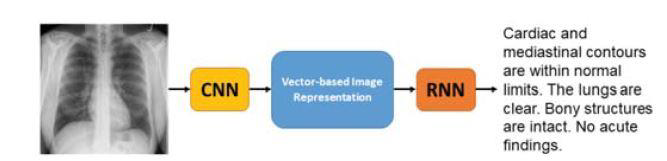
\includegraphics[width=10cm,height=10cm,keepaspectratio]{Encoder-Decoder}
    \end{center}
    \caption{Schema a blocchi di un framework encoder-decoder}
    \label{fig:econder-decoder}
\end{figure}


Il codificatore ha la forma di una rete neurale convoluzionale (CNN) che codifica le immagini DICOM, mentre il decodificatore è una rete neurale ricorrente a più stadi (RNN) che traduce le caratteristiche dell'immagine medica in un referto radiologico.\\
In questo caso viene quindi analizzato un framework codificatore-decodificatore, dove le caratteristiche dell'immagine globale vengono prima estratte utilizzando la CNN e quindi inserite in un LSTM (Long short-term memory) per generare una sequenza di parole. Quando si applica la struttura del codificatore-decodificatore alla generazione di referti di radiologia, l'attività può essere considerata come la traduzione di immagini mediche in referti di radiologia.\\
La figura \ref{fig:LSTM} mostra il diagramma di questo approccio alla generazione di report da immagini mediche. Per generare referti radiologici da immagini mediche, viene fornita un'immagine di input $I$ e il modello dovrebbe generare una sequenza di parole $y = (y_1, y_2, . . . ,y_N)$, dove $y$ denota la descrizione sotto forma di referto radiologico e $y_1 . . .y_N$ denotano le parole nella relazione.\\
Dato un set di allenamento $D = (I, y)$ che consiste in $(I, y)$ coppie, dove $I$ rappresenta una data immagine medica e $y$ rappresenta un referto radiologico accompagnato per l'immagine sotto di $y = (y_1, y_2, . . . ,y_N)$, il modello viene addestrato rispetto ai suoi parametri $\theta$ al fine di massimizzare un modello probabilistico $p_{\theta}(y_1, y_2, . . . , y_N|I)$

\begin{figure}[h!]
    \begin{center}
        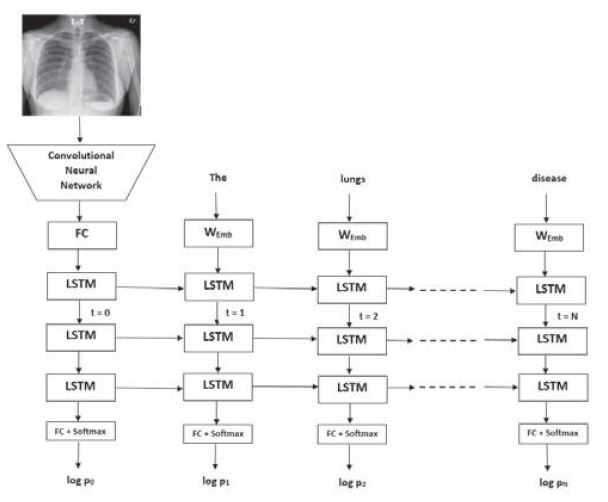
\includegraphics[width=10cm,height=10cm,keepaspectratio]{LSTM}
    \end{center}
    \caption{Un framework Encoder-Decoder per la generazione di referti radiologici da immagini mediche. t = 0, · · · , t = N rappresentano le iterazioni della ricorrenza LSTM.}
    \label{fig:LSTM}
\end{figure}


\subsubsection{Encoder}
Le reti neurali convoluzionali (CNN) sono comunemente utilizzate per le rappresentazioni di immagini in quanto hanno la capacità di catturare caratteristiche a vari livelli di astrazione. Le CNN hanno mostrato prestazioni all'avanguardia nella classificazione delle immagini e nel riconoscimento degli oggetti. I livelli in una CNN includono livelli convoluzionali, livelli di pooling e livelli completamente connessi. 
In questo framework, viene utilizzato il modello Inception-v3 di Google come codificatore perché ha una struttura significativamente più profonda e grazie ai blocchi Inception apprende una rappresentazione semanticamente ricca delle immagini.

\subsubsection{Decoder}
Le reti neurali ricorrenti (RNN) sono reti neurali specializzate che eccellono nell'apprendimento e nell'elaborazione di dati sequenziali come testo e parlato. Gli RNN sono generalmente addestrati dalla retropropagazione nel tempo, il che può portare a problemi di gradienti evanescenti ed esplosivi. Due degli RNN più popolari e importanti che superano questi problemi sono Long-Short Term Memory (LSTM) e Gated Recurrent Unit (GRU). In questo caso, come si può vedere dalla Figura \ref{fig:LSTM}, viene utilizzata una LSTM, che a differenza delle reti neurali feedforward standard, ha connessioni di feedback. Può elaborare non solo singoli punti dati (come immagini), ma anche intere sequenze di dati (come voce o video).

\subsection{Formazione del modello}
Il framework, quindi, è costituito da un codificatore che trasforma l'immagine in una rappresentazione vettoriale e da un decodificatore che trasforma il vettore dell'immagine codificata in una sequenza di parole.\\
Quindi una CNN viene solitamente impiegata come codificatore per estrarre una rappresentazione globale di immagini e il decodificatore è solitamente un RNN che modella il $p(S_t|I, S_0, S_1, . . . ,S_{t-1})$, e genera le frasi corrispondenti.\\
L'obiettivo generale del framework encoder-decoder è trovare la sequenza di parole (frasi) più probabile che descriva una data immagine. Durante l'addestramento, si vuole trovare il modello $\theta^*$ che soddisfa l’equazione 1:

\begin{equation}
{\displaystyle \theta^* =  \arg\max \sum\limits_{(I, S)} \log p(S | I; \theta)},
\end{equation}

dove $\theta$ sono i parametri del modello, $I$ è l'immagine medica di input, e $S$ è il rapporto di verità fondamentale corrispondente all'immagine. La probabilità della descrizione corretta $S$ per una data immagine $I$ può essere modellato come la probabilità congiunta sulle sue parole $S_0, S_1, … ,S_{t-1}$ come indicato nell'equazione 2:

\begin{equation}
{\displaystyle \log p(S|I) =  \sum\limits_{t = 0}^{N} \log p(S_t | I, S_0, S_1, ..., S_{t-1})}
\end{equation}

dove $S_0$, $S_1$, $S_{t-1}$ denotano le parole nell'immagine descrizione. $S_0$ denota uno speciale token $<start>$ e $S_N$ denota uno speciale token $<end>$.

\subsection{Analisi e metriche}
Quando si addestra un algoritmo per un progetto di ricerca per la pratica clinica, è fondamentale comprendere chiaramente le metriche utilizzate per valutare le prestazioni del compito. Per ogni attività di visione artificiale vengono definite metriche specifiche, che possono differire da un obiettivo clinico. Le metriche calcolano i punteggi di somiglianza della didascalia prevista.\\
Il compito di classificazione è strettamente correlato al comune compito interpretativo radiologico di fornire una diagnosi dalle immagini. Di conseguenza, per questa attività, le metriche di apprendimento automatico sono molto simili alle consuete metriche dei test diagnostici riportate in radiologia diagnostica.

\subsection{Distribuzione}
Il deployment si riferisce all'implementazione di una soluzione sviluppata localmente su una scala più ampia, ad esempio a livello di istituto o all'interno di una rete sanitaria. Questo processo richiede una chiara definizione delle specifiche del modello, in termini di prestazioni o di ingegneria del software (ad esempio, configurazioni, versioni, test di unità o requisiti istituzionali specifici).\\
A seconda dell'evoluzione delle metriche delle prestazioni e della valutazione visiva nel tempo, un modello può essere riaddestrato utilizzando dati aggiuntivi per aggiornare dinamicamente le sue prestazioni.
Inoltre, viene consigliato di memorizzare i pesi ottenuti dopo l'allenamento separatamente dall'architettura di rete ai normali checkpoint. Ciò consente aggiornamenti e versioni più semplici, purché l'architettura di rete rimanga identica.\\
Da un punto di vista pratico, l'integrazione dei modelli nelle procedure di routine può essere impegnativa in termini di portabilità, accessibilità dei dati e preelaborazione. È quindi necessario definire se la soluzione sviluppata è destinata ad essere integrata in un'infrastruttura esistente o utilizzata come applicazione standalone. Durante la prima fase di implementazione è possibile adottare un approccio containerizzato come quello proposto da Docker o Kubernetes e applicazioni web-based (REST-API) per l'implementazione successiva.\\
Per soddisfare al meglio queste sfide di integrazione, stanno rapidamente emergendo i mercati delle applicazioni di intelligenza artificiale che offrono un'ampia varietà di strumenti con un'interfaccia utente unificata per i radiologi e un'interfaccia di programmazione delle applicazioni (API) generica per gli sviluppatori. Questo livello commerciale tra i fornitori PACS e le applicazioni di intelligenza artificiale può potenzialmente consentire un'implementazione clinica, una convalida e un'usabilità più rapide.\cite{montagnon2020deep}

\section{Analisi e conclusioni}
In questa fase di analisi ho cercato di confrontare alcuni casi che ho trovato in letteratura: sono andato alla ricerca di quali potessero essere le invarianti e le versatilità tra loro in modo da centrare il nostro obiettivo.\\

\subsection{I dati}
La cosa principale che è comune a tutti è il la struttura del set di dati: set di dati formato sempre da immagine DICOM e/o annotazione.\\
Ovviamente alcuni input devono essere scartati perché non presentano le caratteristiche di cui abbiamo bisogno.\\
Per superare i problemi di privacy sulla violazione dei dati, una potenziale soluzione potrebbe essere quella di eseguire la formazione locale di più modelli e condividere i pesi, una strategia nota come apprendimento federato o distribuito, o, come detto precedentemente, grazie al Transfer Learning.\\
\\
La creazione di grandi set di dati medici di alta qualità è impegnativa e costosa, a causa delle risorse necessarie per la raccolta dei dati e del tempo necessario per l'annotazione. Per affrontare queste limitazioni, sono state proposte alcune strategie di formazione specifiche o architetture di modelli, come l'etichettatura debole o l'apprendimento a pochi colpi.
\\
In generale, lo sviluppo di algoritmi di intelligenza artificiale generalizzabili nell'imaging medico richiede set di dati statisticamente alimentati nell'ordine di centinaia di migliaia o milioni, il che è problematico, data la scarsa disponibilità
dei dati.\\
In alcuni modelli, proprio per questa limitazione, viene eseguito un aumento dei dati di addestramento.\\
Una soluzione parziale per questo problema può essere l'apprendimento semisupervisionato. Sono necessari
set di dati completamente annotati per l'apprendimento supervisionato, mentre l'apprendimento semisupervisionato
utilizza una combinazione di immagini annotate e non annotate per addestrare un algoritmo.
L'apprendimento semi-supervisionato può consentire un numero limitato di casi annotati; tuttavia, sono ancora 
necessari grandi set di dati di immagini non annotate.\\
Un'altra potenziale soluzione futura per aumentare la dimensione del campione di dati potrebbe essere la generazione di dati 
sintetici attraverso reti generative avversarie. Le reti generative avversarie hanno il potenziale per sintetizzare un numero
illimitato di immagini realistiche di alta qualità che possono essere aggiunte ai set di dati di addestramento per lo sviluppo di 
algoritmi di rilevamento e classificazione. Tuttavia, sono disponibili prove limitate, specialmente quando sono presenti anomalie nelle immagini.\\
L'aumento dell'immagine sarebbe preferibile per aumentare il livello di robustezza del modello.
Anche se viene esaminato lo stesso paziente, le immagini non sarebbero identiche tra gli esami a causa di lievi differenze di posizionamento. 
Pertanto, l'uso di immagini ruotate o spostate parallelamente renderebbe il modello robusto per lievi differenze nelle posizioni del paziente. A volte vengono utilizzate anche immagini speculari. L'uso di immagini con rumore aggiunto sarebbe utile per rendere il modello robusto per diversi gradi di rumore dell'immagine.\\

Come già detto precedentemente, un approccio potrebbe differire da un altro anche per le strategie di campionamento del set di dati:
\begin{itemize}
    \item Addestramento, convalida e test
    \item Convalida incrociata k-fold
\end{itemize}
Tuttavia, il primo (Figura \ref{fig:data-sampling-radiology}) è quello più utilizzato, poiché il processo di formazione richiede un'enorme quantità di calcoli.\\

\begin{figure}[h!]
    \begin{center}
        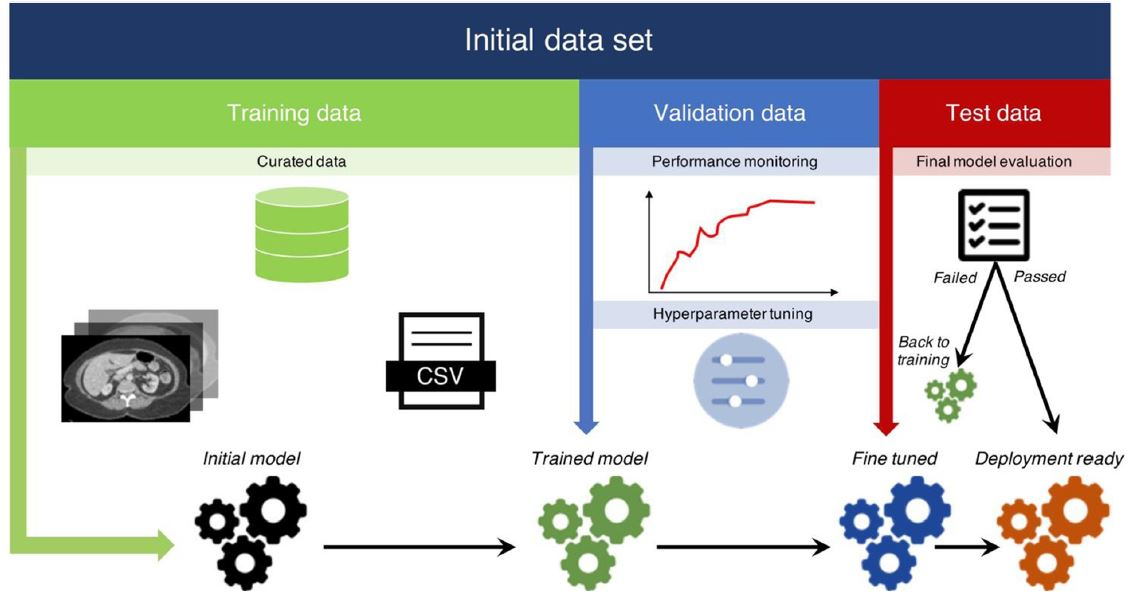
\includegraphics[width=10cm,height=10cm,keepaspectratio]{Data_radiology}
    \end{center}
    \caption{Divisione del set di dati in set di dati di addestramento, convalida e test}
    \label{fig:data-sampling-radiology}
\end{figure}

\subsection{Il modello}
Per estrarre le caratteristiche dall’immagine viene sempre utilizzata un CNN per le sue elevate prestazioni nel riconoscimento delle immagini. La capacità delle CNN di apprendere complesse relazioni spaziali e imparare modelli basati su pixel sottili e intricati li rendono perfetti strumenti per apprendere dalle immagini radiologiche. \\
\\
Per quanto riguarda l'estrazione del testo, invece, le tecniche di elaborazione del linguaggio naturale (NLP) possono essere una chiave per analizzare con successo i referti radiologici per estrarre risultati e raccomandazioni clinicamente importanti. La programmazione neuro-linguistica (PNL) ha già mostrato il potenziale per automatizzare il compito di classificare i report di imaging in un modo che potrebbe informare le decisioni relative all'utilizzo e all'adeguatezza dell'imaging medico \cite{banerjee2019comparative}.\\
Una classe di architetture di reti neurali, le reti neurali ricorrenti (RNN), ha recentemente attirato molta attenzione da parte dei ricercatori per la modellazione di sequenze e ha dimostrato di funzionare bene nella risoluzione di vari compiti di PNL grazie alla loro capacità di gestire input di lunghezza variabile e uscita.\\
Sebbene RNN sia teoricamente un modello potente per codificare informazioni sequenziali, in pratica spesso soffre dei problemi di sfumatura/esplosione del gradiente mentre apprende le dipendenze a lungo raggio. Le reti LSTM e GRU sono note per essere rimedi efficaci a questi problemi.\\
Le estensioni più popolari di RNN sono, appunto, Long Short-Term Memory (LSTM) e la Gated Recurrent Unit (GRU).
LSTM utilizza blocchi di memoria per salvare lo stato temporale della rete e porte per monitorare il flusso di informazioni. D'altra parte, GRU è una forma più leggera di RNN rispetto a LSTM in termini di topologia, spese di calcolo e complessità. Al momento, i ricercatori devono scegliere tra il modello più veloce offerto da GRU che necessita di meno parametri o il modello più performante fornito da LSTM che contiene dati sufficienti e potenza di calcolo.\\

\subsubsection{Tipi di apprendimento}
La Figura \ref{fig:type-of-learning} illustra i tipi di apprendimento: apprendimento supervisionato, semi-supervisionato e non supervisionato.\\
Per l'apprendimento supervisionato, deve essere disponibile uno standard di riferimento per tutti i casi.\\
\\
Per l'apprendimento semi-supervisionato, è disponibile uno standard di riferimento solo per un sottoinsieme di materie. L'apprendimento semi-supervisionato, che si basa su una combinazione di dati etichettati e non etichettati, generalmente ottiene risultati migliori rispetto all'apprendimento supervisionato che si basa solo sul sottoinsieme di dati etichettati. Questo processo di apprendimento combina tecniche non supervisionate e supervisionate.\\
\\
Per l'apprendimento non supervisionato, non è disponibile uno standard di riferimento. In questo contesto, gli algoritmi non supervisionati hanno lo scopo di stabilire una rappresentazione efficiente del set di dati iniziale (ad esempio, clustering attraverso proprietà statistiche, densità o distanze del set di dati). Tale nuova rappresentazione può costituire un primo passo prima della formazione del modello supervisionato, consentendo prestazioni migliori.\\

\begin{figure}[h!]
    \begin{center}
        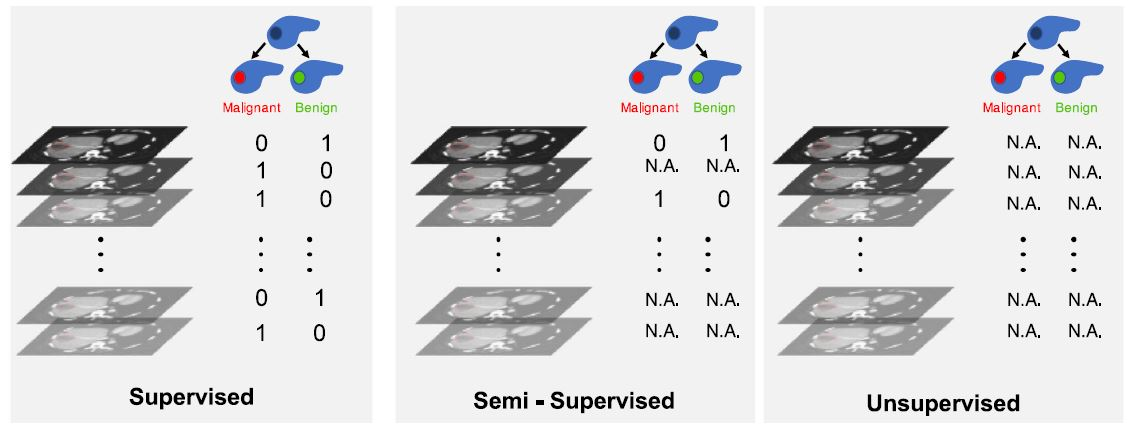
\includegraphics[width=12cm,height=12cm,keepaspectratio]{Type-of-learning}
    \end{center}
    \caption{Tipi di apprendimento. N.A. indica informazioni non disponibili}
    \label{fig:type-of-learning}
\end{figure}


Inoltre è possibile trovare alcuni modelli (es: nel framework r.AID.ologist \cite{r.AID.ologist}) concepiti come modello di ragionamento basato sui casi (Case-Based Reasoning - CBR), alimentato da diversi modelli di deep learning che sono stati inclusi per migliorarne le prestazioni, oltre a fornire funzionalità aggiuntive.
Sebbene CBR sia integrato come un ciclo continuo, le sue sottoparti sono progettate per essere completamente modulari, quindi possono essere facilmente sostituite per adattarsi a nuovi dati.

Il ragionamento basato su casi (CBR) è il processo di risoluzione di nuovi problemi basandosi sulle soluzioni di problemi anteriori ed è stato formalizzato, per il ragionamento automatico, come un processo suddiviso in quattro fasi:
\begin{enumerate}
\item Recupero: Dato un problema, recuperare in memoria dei casi rilevanti (ricordi) per risolverlo. Un caso è composto da un problema, la soluzione e tipicamente alcune annotazioni su come si è arrivati alla soluzione.
\item Riutilizzo: Mappare la soluzione del caso precedente al problema attuale. Ciò può comportare alcune modifiche al caso precedente per adattarlo al caso attuale.
\item Revisione: Avendo mappato la soluzione precedente al caso attuale, bisogna provare la nuova soluzione (nel mondo reale o con una simulazione) e, se necessario rivedere la nuova soluzione.
\item Conservazione: Dopo che la soluzione è stata adattata al problema attuale, memorizzare l'esperienza come nuovo caso.
\end{enumerate}

\subsection{Conclusioni}
Il Deep Learning mostra grandi promesse in radiologia, come dimostrato dalla diversità delle applicazioni e dalle prestazioni riportate in una varietà di compiti di visione artificiale \cite{montagnon2020deep}.\\
Poiché le applicazioni mediche sono numerose e le soluzioni tecniche sono facilmente accessibili, la parte che richiede più tempo è la creazione di set di dati (raccolta e cura di dati), seguito dalla messa a punto del modello attraverso l'ottimizzazione degli iperparametri.\\
Su scala multi-istituzionale, la grande quantità di dati condivisi disponibili costituisce una grande opportunità per la formazione di modelli complessi. I limiti principali sono la disponibilità di annotazioni esperte, il raggruppamento di dati su più siti e la necessità di una cura dei dati per ottenere un set di dati di alta qualità. 


\chapter{Demand forecasting}
La previsione della domanda è uno dei problemi principali delle catene di approvvigionamento. Mira ad ottimizzare le scorte, ridurre i costi e aumentare le vendite, i profitti e la fedeltà dei clienti. A tal fine, i dati storici possono essere analizzati per migliorare la previsione della domanda utilizzando vari metodi come tecniche di apprendimento automatico, analisi di serie temporali e modelli di deep learning.\\
In questo studio viene analizzato il workflow della previsione della domanda con i relativi modelli. 

\section{Overview}
Poiché la concorrenza aumenta di giorno in giorno tra i rivenditori sul mercato, le aziende stanno concentrando più tecniche di analisi predittiva per ridurre i costi e aumentare la produttività e il profitto.\\
Esistono diversi tipi di previsione della domanda: \cite{towards:demandForecast}
\begin{itemize}
    \item A breve termine (viene effettuato per un periodo più breve da 3 mesi a 12 mesi). 
    \item Da medio a lungo termine (in genere viene effettuato da più di 12 mesi a 24 mesi in anticipo (36-48 mesi in alcune attività)).
    \item Livello aziendale interno (questo tipo di previsione si occupa delle operazioni interne dell'azienda come categoria di prodotto, divisione vendite, divisione finanziaria e gruppo di produzione)
    \item Passivo (Si effettua per imprese stabili con piani di crescita molto conservativi. Semplici estrapolazioni di dati storici vengono effettuate con ipotesi minime.)
    \item Attivo (viene eseguito per ridimensionare e diversificare le aziende con piani di crescita aggressivi in termini di attività di marketing, espansione del portafoglio di prodotti e considerazione delle attività della concorrenza e dell'ambiente economico esterno).
\end{itemize}

I rivenditori in diversi settori sono alla ricerca di soluzioni automatizzate di previsione della domanda e rifornimento che utilizzino big data e tecnologie di analisi predittiva. \\
I metodi di previsione tradizionali si basano su approcci di previsione basati su serie temporali. Questi approcci di previsione prevedono la domanda futura in base a dati di serie temporali storiche, ovvero una sequenza di punti dati misurati a intervalli successivi nel tempo.\\
I metodi di previsione dell'apprendimento automatico possono utilizzare una grande quantità di dati e funzionalità correlate alla domanda e prevedere la domanda e i modelli futuri utilizzando diversi algoritmi di apprendimento. Tra molti metodi di apprendimento automatico, i metodi di deep learning (DL) sono diventati molto popolari e sono stati recentemente applicati a molti campi come il riconoscimento di immagini e parole, l'elaborazione del linguaggio naturale e la traduzione automatica. 

\section{Workflow}
In questo caso ho utilizzato un approccio differente dal precedente. Qui non ho analizzato un caso specifico, ma sono riuscito a catturare le possibili generalità del caso. Siccome in letteratura sono state trovate maggiori informazioni riguardo la parte di modello utilizzato, quella parte verrà descritta con maggiore dettaglio rispetto al pretrattamento dei dati.

\subsection{Raccolta dati}
Questo primo processo include i seguenti passaggi: \cite{mobidev:demandForecast}
\begin{enumerate}
    \item Raccogliere i dati disponibili
    \item Esaminare brevemente la struttura dei dati, l'accuratezza e la coerenza
    \item Eseguire alcuni test e progetti pilota sui dati
    \item Guardare attraverso un riepilogo statistico
\end{enumerate}

In questo caso studio il tipo di dato può essere molto differente in base all'obiettivo aziendale. Distinguiamo i dati in:
\begin{itemize}
    \item Strutturati
    \item Non strutturati
\end{itemize}

Nei dati strutturati possiamo trovare dati interni come i dati di vendita e-commerce, le transazioni di vendita, gli ordini d'acquisto, le proprie informazioni POS e dati esterni come tempo metereologico, spedizioni/ricevute del negozio del cliente, le informazioni POS cliente e dati sindacati di terze parti.\\
Nei dati non strutturati possiamo trovare dati interni come siti web, recensioni, campagne di marketing, app, dispositivi in negozio e dati esterni come social media, stream di click, IoT, dispositivi di geolocalizzazione, video, linguaggio naturale.\\
La selezione delle giuste caratteristiche di input per la fase di formazione è fondamentale. In questo contesto, ogni caratteristica rappresenta una variabile di input che influenza l'esito della previsione. 

\subsection{Comprensione e preelaborazione dei dati}
Indipendentemente da ciò che vorremmo prevedere, la qualità dei dati è una componente fondamentale di una previsione accurata della domanda.

\subsubsection{Parametri di qualità dei dati}
Quando si costruisce un modello di previsione, i dati vengono valutati in base ai seguenti parametri:
\begin{itemize}
    \item Consistenza
    \item Precisione
    \item Validità
    \item Rilevanza
    \item Accessibilità
    \item Completezza
    \item Livello di dettaglio
\end{itemize}

\subsubsection{Preelaborazione dei dati}
In realtà, i dati raccolti dalle aziende spesso non sono ideali. Questi dati di solito devono essere puliti, analizzati per lacune e anomalie, verificati per pertinenza e ripristinati.
La preelaborazione può essere applicata in tre forme: adeguamenti stagionali, log o trasformazioni di potenza e rimozione della tendenza \cite{makridakis2018statistical}.
\begin{itemize}
    \item Dati originali: non viene applicata alcuna preelaborazione.
    \item Trasformazione dei dati: ai dati originali viene applicato il log o la trasformazione di potenza Box-Cox (vedi appendice) per ottenere la stazionarietà nella varianza.
    \item Destagionalizzazione dei dati: i dati sono considerati stagionali se esiste un coefficiente di autocorrelazione significativo al lag=12 (dimensione del ritardo). In tal caso i dati vengono destagionalizzati utilizzando il classico approccio di decomposizione moltiplicativa. L'addestramento dei pesi ML, o l'ottimizzazione dei metodi statistici, viene successivamente effettuato sui dati destagionalizzati. I pronostici ottenuti vengono poi ristagionalizzati per determinare i pronostici finali. Ciò non avviene nel caso dei metodi ETS e ARIMA (i modelli classici utilizzati nella statistica) poiché includono modelli stagionali, selezionati utilizzando test relativi e criteri informativi che si occupano direttamente della stagionalità e della complessità del modello.
    \item Detrending dei dati: viene eseguito un test di Cox-Stuart \cite{cox1955some} per stabilire se sia necessario utilizzare un trend lineare deterministico, o in alternativa un primo differenziamento, per eliminare il trend dai dati e ottenere la stazionarietà nella media.
    \item Combinazione dei tre precedenti: i vantaggi delle singole tecniche di preelaborazione vengono applicati simultaneamente per regolare i dati originali.
\end{itemize}

Una volta che i dati sono stati puliti, generati e verificati per pertinenza, vengono strutturati in un modulo completo.\\
La comprensione dei dati è il compito successivo una volta completate la preparazione e la strutturazione. Non è ancora un modello, ma è un modo eccellente per comprendere i dati tramite la visualizzazione. 
Prima di iniziare a creare modelli, bisogna dividere il set di dati per l'addestramento, la convalida e il test, come si può vedere nella Figura \ref{fig:data-split-forecast}.

\begin{figure}[h!]
    \begin{center}
        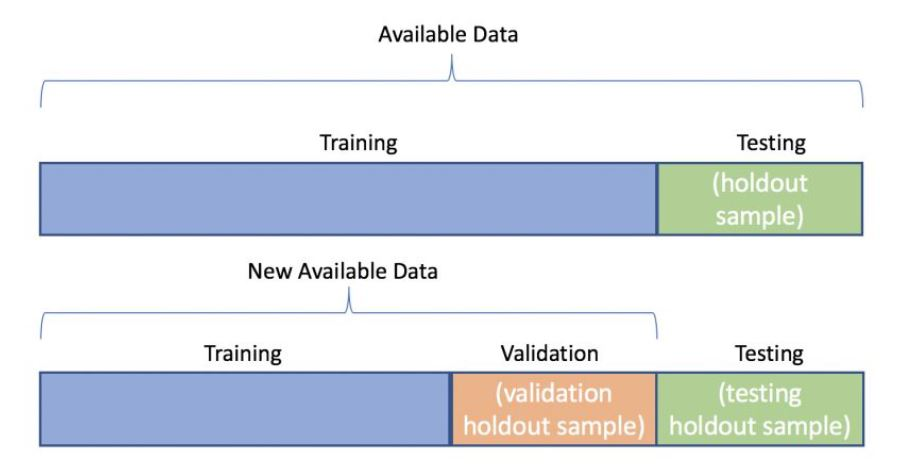
\includegraphics[width=10cm,height=10cm,keepaspectratio]{Data_forecast}
    \end{center}
    \caption{Esempio di suddivisione dei dati}
    \label{fig:data-split-forecast}
\end{figure}


\subsection{Costruzione del modello}
Non esistono algoritmi di previsione "taglia unica". Spesso, le funzionalità di previsione della domanda consistono in diversi approcci di apprendimento automatico. La scelta dei modelli di apprendimento automatico dipende da diversi fattori, come l'obiettivo aziendale, il tipo di dati, la quantità e la qualità dei dati, il periodo di previsione, ecc.\\
Mostreremo i diversi metodi che utilizzano il ML, in particolare l'approccio per serie temporali, che è quello più utilizzato.

Nei modelli di previsione delle serie temporali, l'approccio classico consiste nel raccogliere dati storici, analizzare questi dati sottostanti e utilizzare il modello per prevedere il futuro. Questi algoritmi sono algoritmi di previsione comunemente usati nel dominio di previsione della domanda di serie temporali.

\subsubsection{Perceptron multistrato (MLP)}
Il perceptron multistrato (spesso chiamato semplicemente rete neurale) è una delle architetture di rete più popolare oggi in uso sia per la classificazione che per la regressione. Il MLP è dato come segue:

\begin{equation}
{\displaystyle \hat{y} = v_0 + \sum\limits_{j=1}^{NH} v_jg(w_{j}^{T}x')} ,
\end{equation}

dove $x'$ è il vettore di input $x$, aumentato di 1, cioè $ x' = (1, x^T )^T  $, $w_j$  è il vettore dei pesi per j-esimo nodo nascosto, $v_0, v_1, ..., v_{NH}$ sono i pesi per l'output nodo e $\hat{y}$ è l'output di rete. La funzione g rappresenta l'output del nodo nascosto, ed è data in termini di una funzione di schiacciamento, ad esempio la funzione logistica:
$g(u) = 1/(1 + exp(-u))$. 
L'MLP è un modello fortemente parametrizzato e selezionando il numero di nodi nascosti NH possiamo controllare la complessità del modello. Viene usata una procedura di convalida K-fold per selezionare il numero di nodi nascosti.
Per ottenere i pesi, viene definito l'errore quadratico medio e i pesi vengono ottimizzati utilizzando tecniche di gradiente. Il metodo più noto, basato sul concetto di discesa più ripida, è l'algoritmo di backpropagation. Un metodo di ottimizzazione del secondo ordine chiamato Levenberg Marquardt è generalmente noto per essere più efficiente dell'algoritmo di retropropagazione di base.


\subsubsection{Rete neurale bayesiana (BNN)}
Una rete neurale bayesiana (BNN) è una rete neurale progettata sulla base di una formulazione probabilistica bayesiana (MacKay, 1992a,b). In quanto tali, i BNN sono correlati al concetto di statistica classica della stima dei parametri bayesiani e sono anche correlati al concetto di regolarizzazione come nella regressione della cresta. Le BNN hanno goduto di un'ampia applicabilità in molte aree come l'economia/finanza e l'ingegneria. L'idea di BNN è di trattare i parametri o i pesi di rete come variabili casuali, obbedendo a una distribuzione a priori (vedi appendice). Questa distribuzione è progettata in modo da favorire modelli a bassa complessità, cioè modelli che producono adattamenti lisci. Una volta osservati i dati, viene valutata la distribuzione a posteriori dei pesi e può essere calcolata la previsione della rete. Le previsioni rifletteranno quindi sia l'aspetto di scorrevolezza imposto attraverso l'aspetto di accuratezza precedente che quello di idoneità imposto dai dati osservati.\\
Un concetto strettamente correlato è l'aspetto della regolarizzazione, per cui la seguente funzione obiettivo è costruita e minimizzata

\begin{equation}
{\displaystyle J =\alpha E_D + (1 - \alpha)E_W},
\end{equation}

dove $E_D$ è la somma dei quadrati degli errori nelle uscite di rete, $E_W$ è la somma dei quadrati dei parametri di rete (cioè i pesi) ed $\alpha$ è il parametro di regolarizzazione.
Per l'approccio bayesiano, la scelta tipica del priore (credenze iniziali su un evento in termini di distribuzione di probabilità) è la seguente densità normale che dà più peso ai valori dei parametri di rete più piccoli

\begin{equation}
{\displaystyle p(w) = \left( \frac{1 - \alpha}{\pi} \right)^{\frac{L}{2}} e^{-(1 - \alpha)E_W}},
\label{equation:prior}
\end{equation}

dove $L$ indica il numero di parametri (pesi). Il posteriore è quindi dato da

\begin{equation}
{ \displaystyle p(w \vert D, \alpha) = \frac{p(D \vert w, \alpha)p(w, \alpha)}{p(D, \alpha)} },
\label{equation:posterior}
\end{equation}

dove $D$ rappresenta i dati osservati. Assumendo errori normalmente distribuiti, la densità di probabilità dei dati dati i parametri può essere valutata come

\begin{equation}
{ \displaystyle p(D \vert w, \alpha) = \left( \frac{\alpha}{\pi} \right)^{\frac{M}{2}}  e^{-(1 - \alpha)E_D} },
\label{equation:density}
\end{equation}

dove $M$ è il numero di punti dati di addestramento. Sostituendo le espressioni per le densità in (\ref{equation:prior}) e (\ref{equation:density}) in (\ref{equation:posterior}), otteniamo

\begin{equation}
{ \displaystyle p(w \vert D, \alpha) = c \exp(-J) },
\label{equation:sostitution}
\end{equation}

dove $c$ è una costante di normalizzazione. La costante di regolarizzazione $\alpha$ è anche determinata utilizzando concetti bayesiani, da

\begin{equation}
{ \displaystyle p(\alpha \vert D) = \frac{p(D \vert \alpha)p(\alpha)}{p(D)} }
\label{equation:constant}
\end{equation}

Entrambe le espressioni (\ref{equation:sostitution}) e (\ref{equation:constant}) dovrebbero essere massimizzate per ottenere rispettivamente i pesi ottimali e il parametro $\alpha$. Il termine $p(D \vert \alpha)$ in (\ref{equation:constant}) è ottenuto da un'approssimazione quadratica di $J$ in termini di pesi e quindi integrando i pesi. 

\subsubsection{Reti neurali di regressione generalizzata (GRNN)}
Nadaraya e Watson hanno sviluppato questo modello.
È comunemente chiamato stimatore Nadaraya-Watson o stimatore di regressione del kernel. Nella comunità del machine learning, viene in genere utilizzato il termine rete neurale di regressione generalizzata (o GRNN). Il modello GRNN è un modello non parametrico in cui la previsione per un dato punto di dati x è data dalla media dei risultati target dei punti dati di addestramento in prossimità del punto x dato. La media locale è costruita pesando i punti in base alla loro distanza da $x$, usando alcune funzioni del kernel. La stima è solo la somma ponderata delle risposte osservate (o output target) data da

\begin{equation}
    { \displaystyle \hat{y} = \sum\limits_{m=1}^{M} w_my_m},
\end{equation}

dove i pesi $w_m$ sono dati da


\begin{equation}
    { \displaystyle w_m = \frac{K(\frac{\Vert x-x_m \Vert}{h})}{\sum_{m'=1}^{M}K(\frac{\Vert x-x_{m'} \Vert}{h})}},
\end{equation}

dove $y_m$ è l'output di destinazione per il punto dati di training $x_m$ e $K$ è la funzione del kernel (utilizzando il tipico kernel gaussiano $K(u) = e^{-u^2/2} / \sqrt{2\pi}$).
Il parametro $h$, chiamato larghezza di banda, è un parametro importante in quanto determina la levigatezza dell'adattamento, poiché aumentandolo o diminuendolo controllerà la dimensione della regione di smoothing.

\subsubsection{Regressione K-Nearest Neighbor (KNN)}
Il metodo di regressione K più vicino (KNN) è un metodo non parametrico che basa la sua previsione sugli output di destinazione dei vicini K più vicini del punto di interrogazione dato. Nello specifico, dato un data point, calcoliamo la distanza euclidea tra quel punto e tutti i punti del set di allenamento. Vengono quindi selezionati i dati $K$ più vicini e impostata la previsione come la media dei valori di output target per questi punti $K$. Quantitativamente parlando, sia $I(x)$ l'insieme di $K$ vicini più prossimi del punto $x$. Allora la previsione è data da

\begin{equation}
    {\displaystyle \hat{y} = \frac{1}{K} \sum\limits_{m \in I(x)} y_m}
\end{equation}

dove di nuovo $y_m$ è l'output di destinazione per il punto dati di training $x_m$.
Naturalmente $K$ è un parametro chiave in questo metodo e deve essere selezionato con cura. Un $K$ grande porterà a un adattamento più fluido, e quindi a una varianza inferiore, ovviamente a scapito di un bias maggiore, e viceversa per un $K$ piccolo.

\subsubsection{Regressione del vettore di supporto (SVR)}
La regressione del vettore di supporto è un metodo di successo basato sull'utilizzo di uno spazio di caratteristiche ad alta dimensione (formato trasformando le variabili originali) e penalizzando la conseguente complessità utilizzando un termine di penalità aggiunto alla funzione di errore. Consideriamo prima per l'illustrazione un modello lineare. Quindi, la previsione è data da

\begin{equation}
    {\displaystyle f(x) = w^Tx + b}
\end{equation}

dove $w$ è il vettore del peso, $b$ è il bias e $x$ è il vettore di input. Sia $x_m$ e $y_m$ denotano, rispettivamente, l' m-esimo vettore di input di addestramento e output di destinazione, $m = 1, …, M$. La funzione di errore è data da 

\begin{equation}
    {\displaystyle J = \frac{1}{2}\Vert w \Vert^2 + C\sum\limits_{m=1}^M\vert y_m - f(x_m) \vert_{\epsilon^{\centerdot}} }
\end{equation}

Il primo termine nella funzione di errore è un termine che penalizza la complessità del modello. Il secondo termine è la funzione di perdita $\epsilon-insesitive$, definita come

\begin{equation}
    {\displaystyle \vert y_m - f(x_m) \vert_{\epsilon} = max\{0,|y_m - f(x_m)|-\epsilon\}}
\end{equation}

Non penalizza gli errori sottostanti, consentendo un po' di spazio di manovra per lo spostamento dei parametri per ridurre la complessità del modello. Si può dimostrare che la soluzione che minimizza la funzione di errore è data da

\begin{equation}
    {\displaystyle f(x) = \sum\limits_{m=1}^{M}(\alpha^*_m - \alpha_m)x_m^Tx + b},
\end{equation}

dove $\alpha_m$ e $\alpha_m^\ast$ sono moltiplicatori di Lagrange. I vettori di addestramento che forniscono moltiplicatori di Lagrange diversi da zero sono chiamati vettori di supporto e questo è un concetto chiave nella teoria SVR. I vettori non di supporto non contribuiscono direttamente alla soluzione e il numero di vettori di supporto è una misura della complessità del modello. Questo modello viene esteso al caso non lineare attraverso il concetto di kernel $K$, dando una soluzione

\begin{equation}
    {\displaystyle f(x) = \sum\limits_{m=1}^{M}(\alpha^*_m - \alpha_m)K(x_m^Tx) + b}.
\end{equation}

Un kernel comune è il kernel gaussiano. Si assume che la sua larghezza sia $\sigma K$ (la deviazione standard della funzione gaussiana).


\subsubsection{Rete Neurale Ricorrente (RNN)}
L'RNN semplice, noto anche come rete di Elman, ha una struttura simile all'MLP, ma contiene connessioni di feedback per tenere conto degli stati precedenti insieme all'input corrente prima di produrre l'output o gli output finali.
Questo viene fatto salvando una copia dei valori precedenti del livello contenente i nodi ricorrenti e utilizzandoli come input aggiuntivo per il passaggio successivo. A questo proposito, la rete può esibire un comportamento temporale dinamico per una sequenza temporale.
In questo studio il modello analizzato per implementare la RNN è quello sequenziale. È composto da due livelli, uno nascosto contenente nodi ricorrenti e uno di output contenente uno o più nodi lineari. A causa degli elevati requisiti computazionali, non è molto utilizzata la convalida K-fold per scegliere l'architettura di rete ottimale per serie, ma piuttosto tre nodi di input e sei unità ricorrenti, che formano lo strato nascosto, per tutte le serie temporali del set di dati. 


\subsubsection{Rete neurale di memoria a lungo termine (LSTM)}
La rete LSTM è simile alla RNN discussa sopra ed è stata proposta per evitare il problema della dipendenza a lungo termine. Il vantaggio delle unità LSTM rispetto alle normali unità RNN è la loro capacità di conservare le informazioni per periodi di tempo più lunghi grazie alla loro architettura complessa che consiste in diverse porte con il potere di rimuovere o aggiungere informazioni allo stato dell'unità.
Simile a RNN, il modello analizzato per implementare la rete LSTM è quello sequenziale composto da uno strato nascosto e uno di output. Allo stesso modo, a causa dell'elevato tempo di calcolo, l'architettura del modello è costituita da tre nodi di input, sei unità LSTM che formano lo strato nascosto e un singolo nodo lineare nello strato di output. La funzione di attivazione lineare viene utilizzata prima dell'uscita di tutte le unità e quella del sigmoide rigido per il passo ricorrente. 

\subsection{Formazione del modello}
Una volta sviluppati i modelli di previsione, è il momento di iniziare il processo di formazione. Quando si addestrano i modelli di previsione, i data scientist di solito utilizzano dati storici. Elaborando questi dati, gli algoritmi forniscono modelli addestrati pronti per l'uso.


\subsection{Validazione del modelllo}
Questo passaggio richiede l'ottimizzazione dei parametri del modello di previsione per ottenere prestazioni elevate, utilizzando un metodo di ottimizzazione della convalida incrociata in cui il set di dati di training è suddiviso in dieci parti uguali. I data scientist addestrano modelli di previsione con diversi set di iperparametri. L'obiettivo di questo metodo è capire quale modello ha la previsione più accurata.\\
Mentre alcuni metodi sono migliori per trovare lo schema generale, ignorando i picchi occasionali, altri possono fornire una migliore comprensione degli eventi sporadici. Quando si misurano le prestazioni di un esperimento statistico come una previsione della domanda, ci sono due dimensioni principali:
\begin{enumerate}
    \item Come descrive la tendenza generale del fenomeno
    \item Come si comporta quando incontra possibili valori anomali casuali e rumore
\end{enumerate}

Nell'apprendimento automatico, la definizione del modello e dei suoi parametri/pesi dipende dai criteri di prestazione scelti per la fase di formazione. Criteri diversi determinano pesi del modello diversi.
Le prestazioni dei modelli sono, di solito, valutate utilizzando le metriche statistiche standard RMSE e MAPE. Tuttavia, altre metriche possono essere utili, come l'errore medio (ME) e Il coefficiente di determinazione R2.


\subsection{Miglioramento}
Quando si ricercano le migliori soluzioni aziendali, gli scienziati dei dati di solito sviluppano diversi modelli di apprendimento automatico. Poiché i modelli mostrano diversi livelli di accuratezza, gli scienziati scelgono quelli che soddisfano meglio le loro esigenze aziendali. La fase di miglioramento prevede l'ottimizzazione dei risultati analitici. Ad esempio, utilizzando tecniche di insieme di modelli, è possibile ottenere una previsione più accurata. In tal caso, l'accuratezza viene calcolata combinando i risultati di più modelli di previsione.


\subsection{Distribuzione}
Questa fase presuppone l'integrazione dei modelli di previsione nell'uso della produzione. Si consiglia inoltre di impostare una pipeline per aggregare nuovi dati da utilizzare per le prossime funzionalità di intelligenza artificiale. Ciò può far risparmiare molto lavoro di preparazione dei dati in progetti futuri. In questo modo aumenta anche la precisione e la varietà di ciò che potresti essere in grado di prevedere.


\section{Analisi e conclusioni}
In questa fase di analisi ho cercato di confrontare alcuni casi che ho trovato in letteratura: sono andato a ricercare quali potessero essere le invarianti e le versatilità tra loro.
Le svariate applicazioni della previsione della domanda portano anche a svariati modelli utilizzabili e svariati modi di pretrattare i dati.\\

\subsection{I dati}
I diversi modi di pretrattare i dati dipendono dal tipo di modello utilizzato.\\
Allo stesso tempo nei problemi di classificazione, le prestazioni degli algoritmi di apprendimento dipendono principalmente dalla natura della rappresentazione dei dati.\\

Come visto in precedenza, le modalità di pretrattamento dei dati sono molteplici:
\begin{itemize}
    \item Trasformazione dei dati (log o la trasformazione di potenza Box-Cox).
    \item Destagionalizzazione dei dati.
    \item Detrending dei dati.
    \item Combinazione dei tre precedenti
\end{itemize}

Si è evidenziata inoltre la necessità non solo di considerare l'uso attento dei metodi di preparazione dei dati, ma di testare attivamente più combinazioni diverse di schemi di preparazione dei dati per un dato problema al fine di scoprire cosa funziona meglio, anche nel caso dei metodi classici.\\

\paragraph*{Estrazione delle caratteristiche:}
Potrebbero esserci alcuni problemi a causa dell'enorme quantità di dati. Quando si prova ad utilizzare tutte le funzionalità di tutti i dati, l'algoritmo di deep learning può impiegare persino giorni per completare il suo lavoro a causa della potenza di calcolo limitata. \cite{kilimci2019improved}\\
Quindi per ogni algoritmo è necessario ridurre il numero di caratteristiche e il tempo di calcolo. Per superare questo problema e accelerare le fasi di clustering e modellazione, potrebbe essere utilizzato PCA (Principal Component Analysis) come algoritmo di estrazione delle caratteristiche.\\
PCA è un algoritmo di riduzione delle dimensioni comunemente utilizzato che presenta le caratteristiche più significative. PCA trasforma ogni istanza del dato insieme di dati dallo spazio d dimensionale a un sottospazio dimensionale k in cui il nuovo insieme generato di k dimensioni è chiamato Componenti Principali (PC). Ogni componente principale è diretto ad una varianza massima esclusa la varianza, contabilizzata in tutte le sue componenti precedenti. Di conseguenza, il primo componente copre la massima varianza e così via.\\
In breve, i Componenti Principali sono rappresentati come \cite{kilimci2019improved}
\begin{equation}
    {\displaystyle PC_i = a_1X_1 + a_2X_2 + ...}
\end{equation}

dove $PC_i$ è l'$i$-esimo componente principale, $X_j$ è la $j$-esima caratteristica originale e $a_j$ è il coefficiente numerico per la caratteristica $X_j$.\\
\\
Le caratteristiche per la previsione della domanda dipendono fortemente dall'obiettivo aziendale. Per esempio, la comunità scientifica ha effettuato diversi studi riguardanti le caratteristiche più adeguate per la previsione della domanda idrica \cite{antunes2018short} e si può genericamente concludere che, oltre ai dati storici, il clima e la stagionalità hanno l'impatto più forte sui risultati e possono essere presi in considerazione anche gli sporadici eventi stagionali, come Natale, Pasqua o anche un grande evento sportivo.\\
Quando si parla di stagionalità, essa può essere implementata nell'algoritmo in due modi diversi:
\begin{enumerate}
    \item La periodicità dei dati influenza direttamente il numero di macchine (modelli predittivi) utilizzate nella previsione e, di conseguenza, la quantità di dati utilizzati nell'addestramento di ciascuna macchina. Ad esempio, considerando una periodicità di 24 ore significa che l'algoritmo addestrerà 24 macchine e farà previsioni per un intervallo di 24 ore. Le diverse periodicità da considerare hanno applicazioni diverse e possono avere implicazioni per l'accuratezza delle previsioni.
    \item Identificare e separare diversi modelli nei dati e utilizzare ciascuno di essi come set di dati indipendenti. Questo è noto come clustering e può essere ottenuto utilizzando algoritmi di apprendimento automatico.
\end{enumerate}

\paragraph*{Clustering dei dati:}
Nell'apprendimento non supervisionato, un problema comune è identificare e classificare correttamente un certo numero di classi identiche (cluster) presenti nei dati. All'inizio, il numero di cluster, k, è solitamente sconosciuto e può essere ottenuto eseguendo l'algoritmo di clustering per diversi valori di k e valutando i risultati per ciascun valore.\\
Il numero ottimale di cluster è quello che ottimizza un determinato criterio, come la varianza tra osservazioni nello stesso cluster.
Complessivamente, il numero di cluster e il modo in cui vengono trovati, la formulazione della distanza e l'implementazione dell'algoritmo di clustering stesso sono reciprocamente influenzati e diverse combinazioni di essi produrranno risultati diversi.\\
Qui, l'analisi di clustering può essere utilizzata per verificare la stagionalità e altre relazioni tra i dati di input.\\
\\

\subsection{Il modello}
Come visto in precedenza i modelli da poter utilizzare sono molteplici:
\begin{itemize}
    \item Perceptor multistrato (MLP)
    \item Rete neurale bayesiana (BNN)
    \item Reti neurali di regressione generalizzata (GRNN)
    \item Regressione K-Nearest Neighbor (KNN)
    \item Regressione del vettore di supporto (SVR)
    \item Rete Neurale Ricorrente (RNN)
    \item Rete neurale di memoria a lungo termine (LSTM)
\end{itemize}

Come mostrato in letteratura, tecniche diverse sono più adatte a sistemi diversi. Per questo motivo, non ci si aspetta di trovare una soluzione che si adatti perfettamente a tutti i set di dati o di trovare la soluzione perfetta per ciascuna metodologia. Tuttavia, si prevede di scoprire quali configurazioni del modello testate presentano i migliori risultati.
Inoltre, i vantaggi di ciascuna tecnica possono essere combinati attraverso una strategia ibrida di metodi paralleli, diluendo gli svantaggi.\\
Di seguito riporto altri tre tipi di modelli utilizzati nella previsione della domanda e anche una metodologia proposta in letteratura.

\paragraph*{Radial Basis Functions (RBF):}
RBF è una rete feed-forward con un livello nascosto ed è simile al metodo MLP tranne per il fatto che i nodi hanno una funzione di attivazione localizzata. Più comunemente, le funzioni nodo vengono scelte come funzioni gaussiane, con l'ampiezza della funzione gaussiana che controlla l'uniformità della funzione adattata. Gli output dei nodi sono combinati linearmente per fornire l'output di rete finale.
 
\paragraph*{CART regression trees (CART):}
CART è un modello di classificazione o regressione basato su una partizione gerarchica ad albero dello spazio di input.
Nello specifico, lo spazio di input è suddiviso in regioni locali identificate in una sequenza di scissioni ricorsive. L'albero è costituito da nodi decisionali interni e foglie terminali. Dato un punto dati di test, una sequenza di test lungo i nodi decisionali a partire dal nodo radice determinerà il percorso lungo l'albero fino a raggiungere un nodo foglia. Al nodo foglia, viene effettuata una previsione in base al modello locale associato a quel nodo. Per costruire un albero utilizzando il training set, si inizia dal nodo radice. Si seleziona la variabile (e la sua soglia di suddivisione) la cui suddivisione porterà alla maggiore riduzione dell'errore quadratico medio. Si continuano queste divisioni in modo ricorsivo, fino a quando l'errore quadratico medio raggiunge una soglia accettabile.\\
Una pratica tipica è quella di eseguire una sorta di potatura per l'albero, una volta progettato. Ciò eliminerà i nodi inefficaci e manterrà sotto controllo la complessità del modello. 

\paragraph*{Gaussian Processes (GP):}
Secondo GP, ogni variabile target può essere associata ad una o più variabili casuali normalmente distribuite che formano una distribuzione normale multivariata, emergente combinando le singole distribuzioni di quelle indipendenti. A questo proposito, i processi gaussiani possono fungere da metodo di regressione non parametrico che assume una distribuzione a priori per le variabili di input fornite durante l'addestramento e quindi le combina in modo appropriato utilizzando una misura di somiglianza tra punti (la funzione kernel) per prevedere il valore futuro della variabile di interesse.\\
\\
Oltre ai modelli discussi in precedenza c'è anche l'Ensemble Learning (EL). È una metodologia d'insieme utilizzata per aumentare le prestazioni del sistema utilizzando modelli multipli per ottenere una migliore prestazione predittiva rispetto ai modelli da cui è costituito.
\paragraph*{Ensemble Learning:}
Un sistema di insieme è composto da due parti: \cite{towards:demandForecast}
\begin{itemize}
    \item generazione di insieme
    \item integrazione di insieme.
\end{itemize}
Nella parte di generazione dell'ensemble, viene generato un insieme diversificato di modelli di previsione di base utilizzando metodi o campioni diversi. Nella parte di integrazione, le previsioni di tutti i modelli vengono combinate utilizzando una strategia di integrazione.\\

Descrivo in breve un algoritmo in particolare che si approccia molto a questo caso, e si tratta dell'algoritmo Stacking:\\
Stacking o Stacked Generalization è un algoritmo di apprendimento automatico di insieme. Utilizza un algoritmo di meta-apprendimento per apprendere come combinare al meglio le previsioni di due o più algoritmi di apprendimento automatico di base.\\
L'architettura di un modello di impilamento (stacking model) coinvolge due o più modelli di base, spesso indicati come modelli di livello 0 e un meta-modello che combina le previsioni dei modelli di base indicati come modello di livello 1:
\begin{itemize}
    \item Modelli di livello 0 (modelli base): i modelli si adattano ai dati di addestramento e le cui previsioni vengono compilate.
    \item Modello di Livello 1 (Meta-Modello): modello che apprende come combinare al meglio le previsioni dei modelli base.
\end{itemize}
Il meta-modello è addestrato sulle previsioni fatte dai modelli di base su dati fuori campione. In altre parole, i dati non utilizzati per addestrare i modelli di base vengono inviati ai modelli di base, vengono effettuate previsioni e queste previsioni, insieme agli output previsti, forniscono le coppie di input e output del set di dati di addestramento utilizzato per adattarsi al meta-modello. Gli output dei modelli di base utilizzati come input per il meta-modello possono essere valori reali in caso di regressione e valori di probabilità, valori simili alla probabilità o etichette di classe in caso di classificazione.
La regressione a stack è una tecnica di apprendimento di insieme per combinare più modelli di regressione tramite un meta-regressore. I singoli modelli di regressione vengono addestrati in base al training set completo; quindi, il meta-regressore viene adattato in base agli output - meta-caratteristiche - dei singoli modelli di regressione nell'insieme.\\

\subsection{Conclusioni}
Dopo aver esaminato molti articoli in lettatura, gli studi fatti precedentemente forniscono importanti prove a sostegno del fatto che i metodi classici possono dominare la previsione di serie temporali.\\
Gli autori di alcuni articoli fanno commenti su LSTM e RNN, che sono generalmente ritenuti l'approccio di deep learning per problemi di previsione di sequenza in generale, e in questo caso le loro prestazioni chiaramente scarse nella pratica.\\
\\
\emph{[...] one would expect RNN and LSTM, which are more advanced types of NNs, to be far more accurate than the ARIMA and the rest of the statistical methods utilized.} \cite{makridakis2018statistical}\\
\\
Dicendo anche che gli LSTM sembrano essere più adatti ad adattare o sovradimensionare il set di dati di allenamento piuttosto che a prevederlo.\\
\\
\emph{Another interesting example could be the case of LSTM that compared to simpler NNs like RNN and MLP, report better model fitting but worse forecasting accuracy.} \cite{makridakis2018statistical}\\
\\
Come già detto precedentemente, la letteratura analizzata si concentra molto di più sulla parte di analisi dei modelli, ed è per questo che vengono forniti più dettagli al riguardo rispetto al preprocessamento dei dati, che, come si è visto, può anche essere assente. I modelli da utilizzare sono molti e c'è anche la possibilità di combinare alcuni di questi per migliorare le prestazioni.\\





\chapter{Frameworks}
Gli strumenti di orchestrazione del machine learning vengono utilizzati per automatizzare e gestire i workflow e l'infrastruttura della pipeline, con un'interfaccia semplice e collaborativa. Insieme alla gestione e alla creazione di workflow personalizzati e delle relative pipeline, questi strumenti ci aiutano anche a tracciare e monitorare i modelli per ulteriori analisi.
Gli strumenti di orchestrazione rendono il processo di machine learning più semplice, più efficiente e aiutano i data scientist e i team di machine learning a concentrarsi su ciò che è necessario, piuttosto che sprecare risorse cercando di identificare i problemi prioritari.\\
Come abbiamo detto precedentemente, il nostro scopo è quello di cercare quei framework che meglio si integrano con una piattaforma esistente di gestione di risorse di AI/ML, come AI4EU. La selezione dei framework è data principalmente da questo fattore, ovvero se un framework dovesse essere messo in un ambiente di produzione, come quello di AI4EU: quelli selezionati sono i candidati più sensati, scartando invece quelli utilizzati in ambito di ricerca/accademico.\\
Senza la pretesa di essere completi riportiamo il risultato dell'analisi che è stata eseguita.
È stata eseguita un'analisi astratta, ovvero non sono stati selezionati determinati framework implementandoli, ma solo vedendo quali sono le loro capacità e verificare che siano compatibili con le nostre necessità.\\
La lista di tool che si occupano di framework è molto vasta. Quelli che hanno un utilizzo ampio da parte dei pratictioners e quelli che meglio si adattano ai nostri casi studio sono illustrati di seguito.

\section{MetaFlow}
Metaflow è una libreria Python di facile utilizzo che aiuta scienziati e ingegneri a creare e gestire progetti di data science reali. Metaflow è stato originariamente sviluppato da Netflix per aumentare la produttività dei data scientist che lavorano su un'ampia varietà di progetti, dalle statistiche classiche al deep learning all'avanguardia. \cite{MetaFLow}
Metaflow fornisce un'API unificata allo stack dell'infrastruttura necessario per eseguire progetti di data science, dal prototipo alla produzione, ma non presenta un'interfaccia grafica per visualizzare e gestire i flussi di lavoro.
Purtoppo però MetaFlow non offre una UI per visualizzare e gestire il workflow.\\

\begin{figure}[h!]
    \begin{center}
        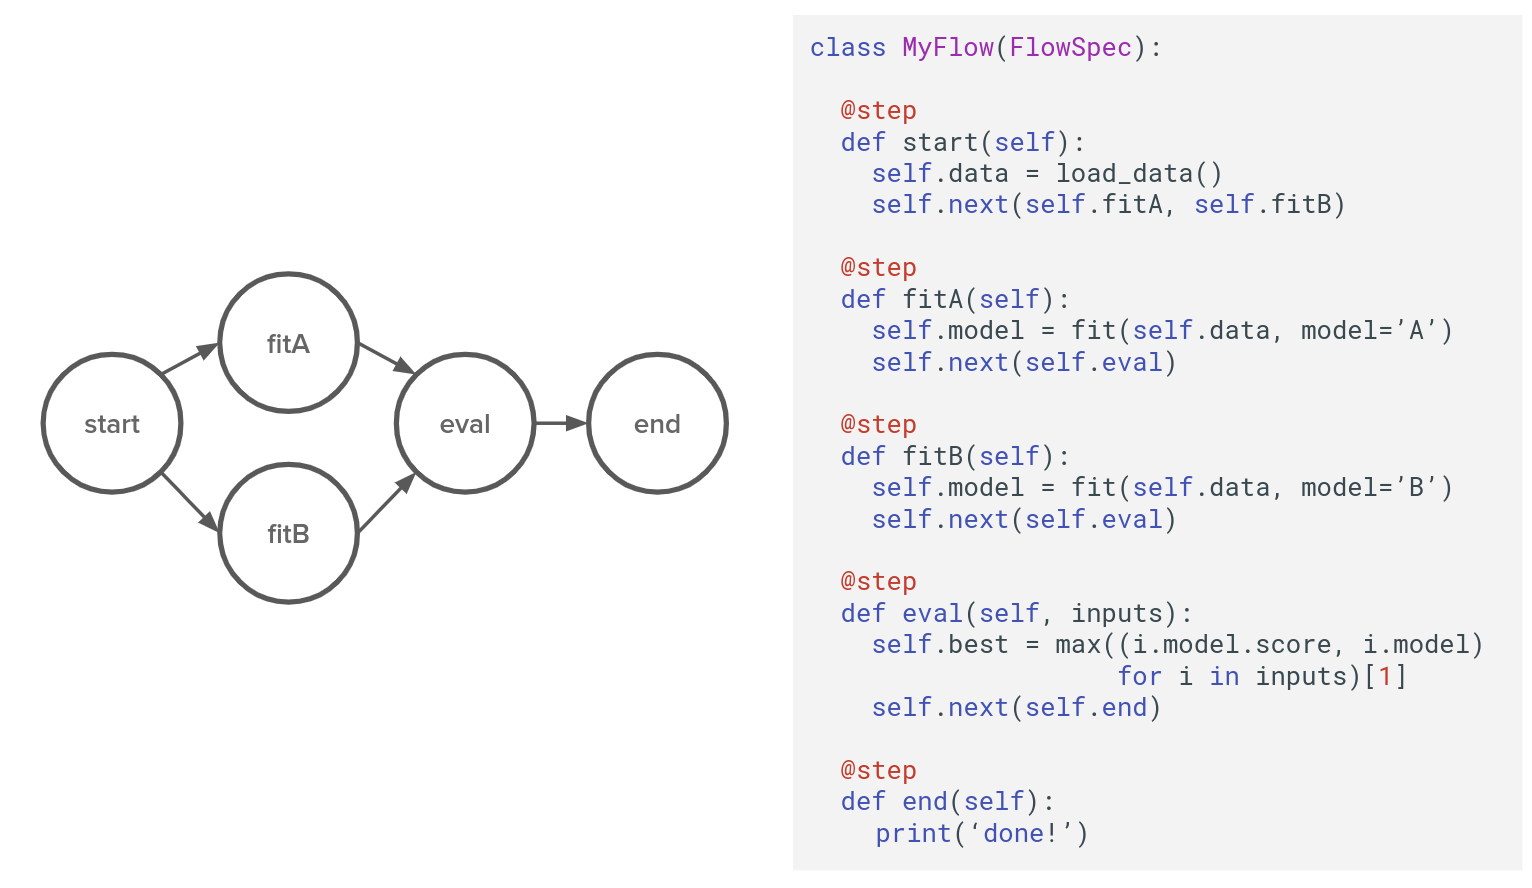
\includegraphics[width=12cm,height=12cm,keepaspectratio]{MetaFlow}
    \end{center}
    \caption{Esempio di addestramento di due versioni di un modello in parallelo e scelta di quella con il punteggio più alto}
    \label{fig:ex-MetaFlow}
\end{figure}

Con questo framework, i data scientists possono strutturare il proprio flusso di lavoro come un grafico aciclico diretto di passaggi, come illustrato sopra. I passaggi possono essere codice Python arbitrario. In questo esempio ipotetico, il flusso addestra due versioni di un modello in parallelo e sceglie quella con il punteggio più alto. Anche per questo motivo si appresta al nostro caso.\\
Per fare una predizione accurata della domanda, come già detto precedentemente, è conveniente addestrare varie versioni di un modello per scoprire quali configurazioni del modello testate presentano i migliori risultati, o addiritura addestrare in parallelo vari tipi di modello.\\
In superficie, questo non sembra molto. Esistono molti framework esistenti, che consentono l'esecuzione di DAG costituiti da codice Python arbitrario. Il "problema" è nei molti dettagli accuratamente progettati di Metaflow: ad esempio, si noti come nell'esempio sopra i dati e i modelli sono memorizzati come normali variabili di istanza Python. Funzionano anche se il codice viene eseguito su una piattaforma di calcolo distribuita, supportata da Metaflow per impostazione predefinita, grazie all'archivio di artefatti indirizzato al contenuto integrato di Metaflow. In molti altri framework, il caricamento e l'archiviazione degli artefatti è lasciato come esercizio per l'utente, che lo costringe a decidere cosa dovrebbe e non dovrebbe essere mantenuto. Metaflow rimuove questo sovraccarico cognitivo.

\subsection{Vantaggi}
Metaflow segue il dataflow paradigm che modella un programma come un grafo diretto di operazioni. Questo è un paradigma naturale per esprimere le pipeline di elaborazione dei dati, in particolare l'apprendimento automatico.\\
I vantaggi principali di questo framework sono: \cite{MetaFLow}
\begin{itemize}
    \item Fornisce un'API altamente utilizzabile per strutturare il codice come flusso di lavoro, ovvero come grafico diretto dei passaggi (usabilità).
    \item Mantiene un'istantanea immutabile di dati, codice e dipendenze esterne necessarie per eseguire ogni passaggio (riproducibilità).
    \item Facilita l'esecuzione delle fasi in vari ambienti, dallo sviluppo alla produzione (scalabilità, prontezza alla produzione).
    \item Registra i metadati sulle precedenti esecuzioni e rendili facilmente accessibili (usabilità, riproducibilità).
\end{itemize}

E come si può vedere la prontezza della produzione è uno degli aspetti che ci interessa.

\section{ZenML}
ZenML è un framework MLOps estensibile e open source per l'utilizzo di pipeline di Machine Learning pronte per la produzione, in modo semplice. Al suo interno, ZenML organizza le pipeline degli esperimenti dall'acquisizione dei dati alla suddivisione, preelaborazione, formazione, fino alla valutazione dei risultati e persino alla pubblicazione. \cite{ZenML}\\
Sebbene esistano altre soluzioni di pipeline per gli esperimenti di Machine Learning, ZenML si concentra su quanto segue:
\begin{itemize}
    \item Semplicità.
    \item Riproducibilità.
    \item Integrazioni.
\end{itemize}

\begin{figure}[h!]
    \begin{center}
        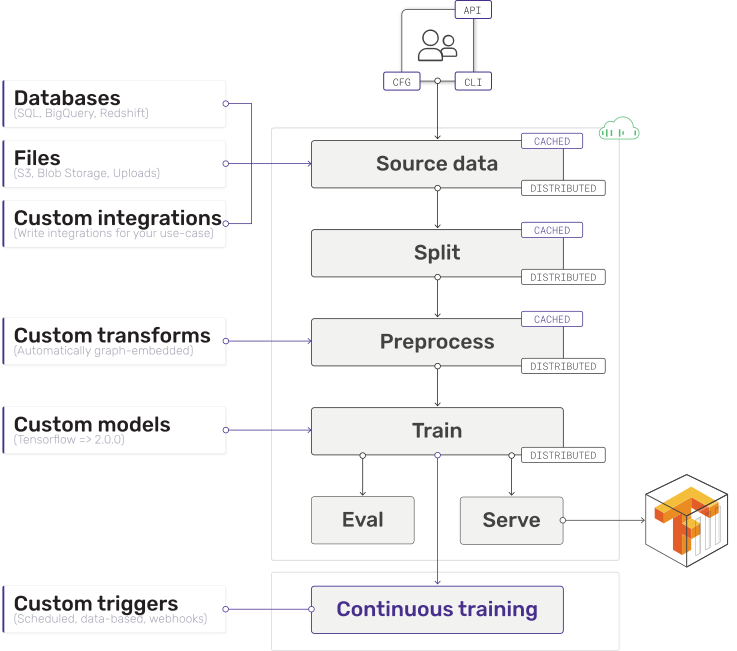
\includegraphics[width=8cm,height=8cm,keepaspectratio]{ZenML-schema}
    \end{center}
    \caption{Pipeline con ZenML}
    \label{fig:ZenML-schema}
\end{figure}

\subsection{Problemi risolti da ZenML}
ZenML risolve il problema di portare in produzione l'apprendimento automatico nei modelli. Da quello che è riportato nella documentazione del sito è conveniente usare ZenML se si lotta con: \cite{ZenML}
\begin{itemize}
    \item Riproduzione dei risultati della formazione in produzione.
    \item Gestione dei metadati ML, inclusi dati, codice e versionamento del modello.
    \item Ottenere (e mantenere) i modelli ML in produzione.
    \item Riutilizzare codici/dati e ridurre gli sprechi.
    \item Mantenimento della comparabilità tra i modelli ML.
    \item Ridimensionamento dell'addestramento/inferenza ML a set di dati di grandi dimensioni.
    \item Mantenimento della qualità del codice insieme alla velocità di sviluppo.
    \item Tenere il passo con il panorama degli strumenti ML in modo coerente.
\end{itemize}

Molto importante per noi è il ridimensionamento del set di dati e, appunto, la facilità del portare i modelli in produzione.\\
Nel caso del demand forecasting, come già detto in precedenza, potrebbe esserci la possibilità di ridurre il set di dati al fine di ridurre anche il tempo di addestramento.\\
\\
Nel caso dell'AI in radiology, il riutilizzo del codice è fondamentale. Come abbiamo visto precedentemente per estrarre le caratteristiche da un'immagine viene sempre utilizzata una CNN: a questo punto quel modulo potrà essere quasi sempre riutilizzato in tutti i casi di estrazione delle caratteristiche da un'immagine.\\

\subsection{Vantaggi}
Elenco di seguito i vantaggi, di ZenML, a cui siamo interessati:
\begin{itemize}
    \item Riproducibilità garantita degli esperimenti di addestramento tramite:
    \begin{itemize}
        \item Dati versione, codice e modelli
        \item Esperimenti monitorati automaticamente
        \item Configurazioni dichiarative della pipeline
    \end{itemize}
    \item Possibilità di passare rapidamente dall'ambiente locale a quello cloud (ad es. orchestrazione di pipeline su kubernetes)
    \item Astrazioni integrate ed estensibili per:
    \begin{itemize}
        \item Preelaborazione distribuita su grandi set di dati
        \item Lavori di formazione basati su cloud        
        \item Servizio modello
    \end{itemize}
\end{itemize}
Inoltre sono supportati tutti i metodi comuni di preprocessing, comprese le serie temporali.\\
Nel caso dell'AI in radiology, come già detto, è necessario definire se la soluzione sviluppata è destinata ad essere integrata in un'infrastruttura esistente o utilizzata come applicazione standalone. Durante la prima fase di implementazione, è possibile adottare un approccio containerizzato come quello proposto da Docker o Kubernetes.\\
Quindi la possibilità che dà ZenML di passare rapidamente da un ambiente locale a quello cloud come kubernetes gioca a suo vantaggio.

\section{MLRun}
MLRun è un framework MLOps open source che offre un approccio integrativo alla gestione delle pipeline di machine learning dallo sviluppo iniziale allo sviluppo del modello fino alla distribuzione completa della pipeline in produzione. MLRun offre un comodo livello di astrazione per un'ampia varietà di stack tecnologici, consentendo ai data engineer e ai data scientist di definire la funzionalità e i modelli.\cite{MLRun}
\\
\begin{figure}[h!]
    \begin{center}
        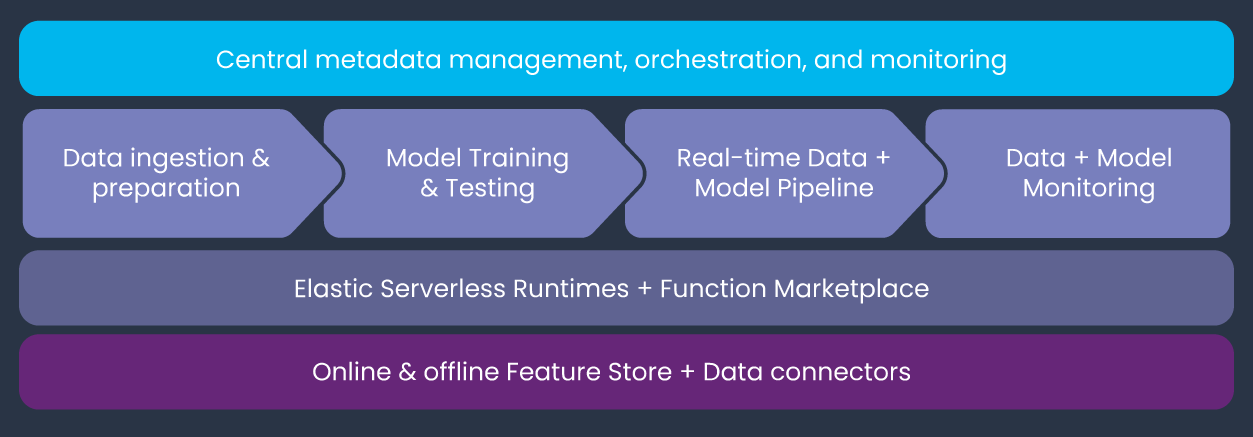
\includegraphics[width=12cm,height=12cm,keepaspectratio]{MLRun}
    \end{center}
    \caption{architettura di MLRun}
    \label{fig:MLRun}
\end{figure}

\subsection{Vantaggi}
MLRun offre i seguenti vantaggi chiave:

\begin{itemize}
    \item Implementazione rapida del codice nelle pipeline di produzione
    \item Ridimensionamento elastico di carichi di lavoro batch e in tempo reale
    \item Gestione delle funzionalità: acquisizione, preparazione e monitoraggio
    \item Funziona ovunque: il tuo IDE locale, multi-cloud o on-premise
\end{itemize}


Per garantire efficienza e scalabilità, è necessario implementare il parallelismo quando possibile. MLRun supporta questo utilizzando due meccanismi: \cite{MLRun}

\begin{enumerate}
    \item Clustering: eseguire il codice su un motore di elaborazione distribuito (come Dask, Spark o Horovod).
    \item Bilanciamento del carico/partizionamento: dividere (partizionare) il lavoro tra più lavoratori.
\end{enumerate}

Le funzioni e le attività MLRun possono accettare iperparametri o elenchi di parametri, distribuire molti worker paralleli e suddividere il lavoro tra i worker distribuiti. L'implementazione del parallelismo è lasciata al runtime. Ogni runtime può avere il proprio metodo di esecuzione delle attività simultanee.\\
MLRun, quindi, supporta il parallelismo. Ad esempio, il codice seguente mostra come utilizzare gli iperparametri per eseguire l'attività di addestramento del modello XGBoost con diverse combinazioni di parametri:
\\
\begin{lstlisting}[caption={Esempio di codice},captionpos=b, label={code:MLRun-code}]
parameters = {
    "eta":       [0.05, 0.10, 0.20, 0.30],
    "max_depth": [3, 4, 5, 6, 8, 10],
    "gamma":     [0.0, 0.1, 0.2, 0.3],
    }

task = NewTask(handler=xgb_train, out_path='/User/mlrun/data').with_hyper_params(parameters, 'max.accuracy')
run = run_local(task)
\end{lstlisting}

Questo codice (\ref{code:MLRun-code}) mostra come indicare a MLRun di eseguire la stessa attività mentre si scelgono i parametri da più elenchi (ricerca a griglia). MLRun quindi registra tutte le esecuzioni, ma contrassegna solo l'esecuzione con perdita minima come risultato selezionato \cite{MLRun}.
\\
Oltre alla implementazione rapida del codice nelle pipeline di produzione, è anche per il parallelismo che MLRun è un ottimo candidato per il nostro scopo. Per quanto riguarda il demand forecasting, data la mole di dati, il parallelismo rappresenta un'ottima soluzione al problema di allenare una rete con tantissimi dati.\\
Un altro vantaggio di MLRun è che ha anche un'interfaccia utente grafica (MLRun Dashbord) per lavorare e visualizzare i dati.
\begin{figure}[h!]
    \begin{center}
        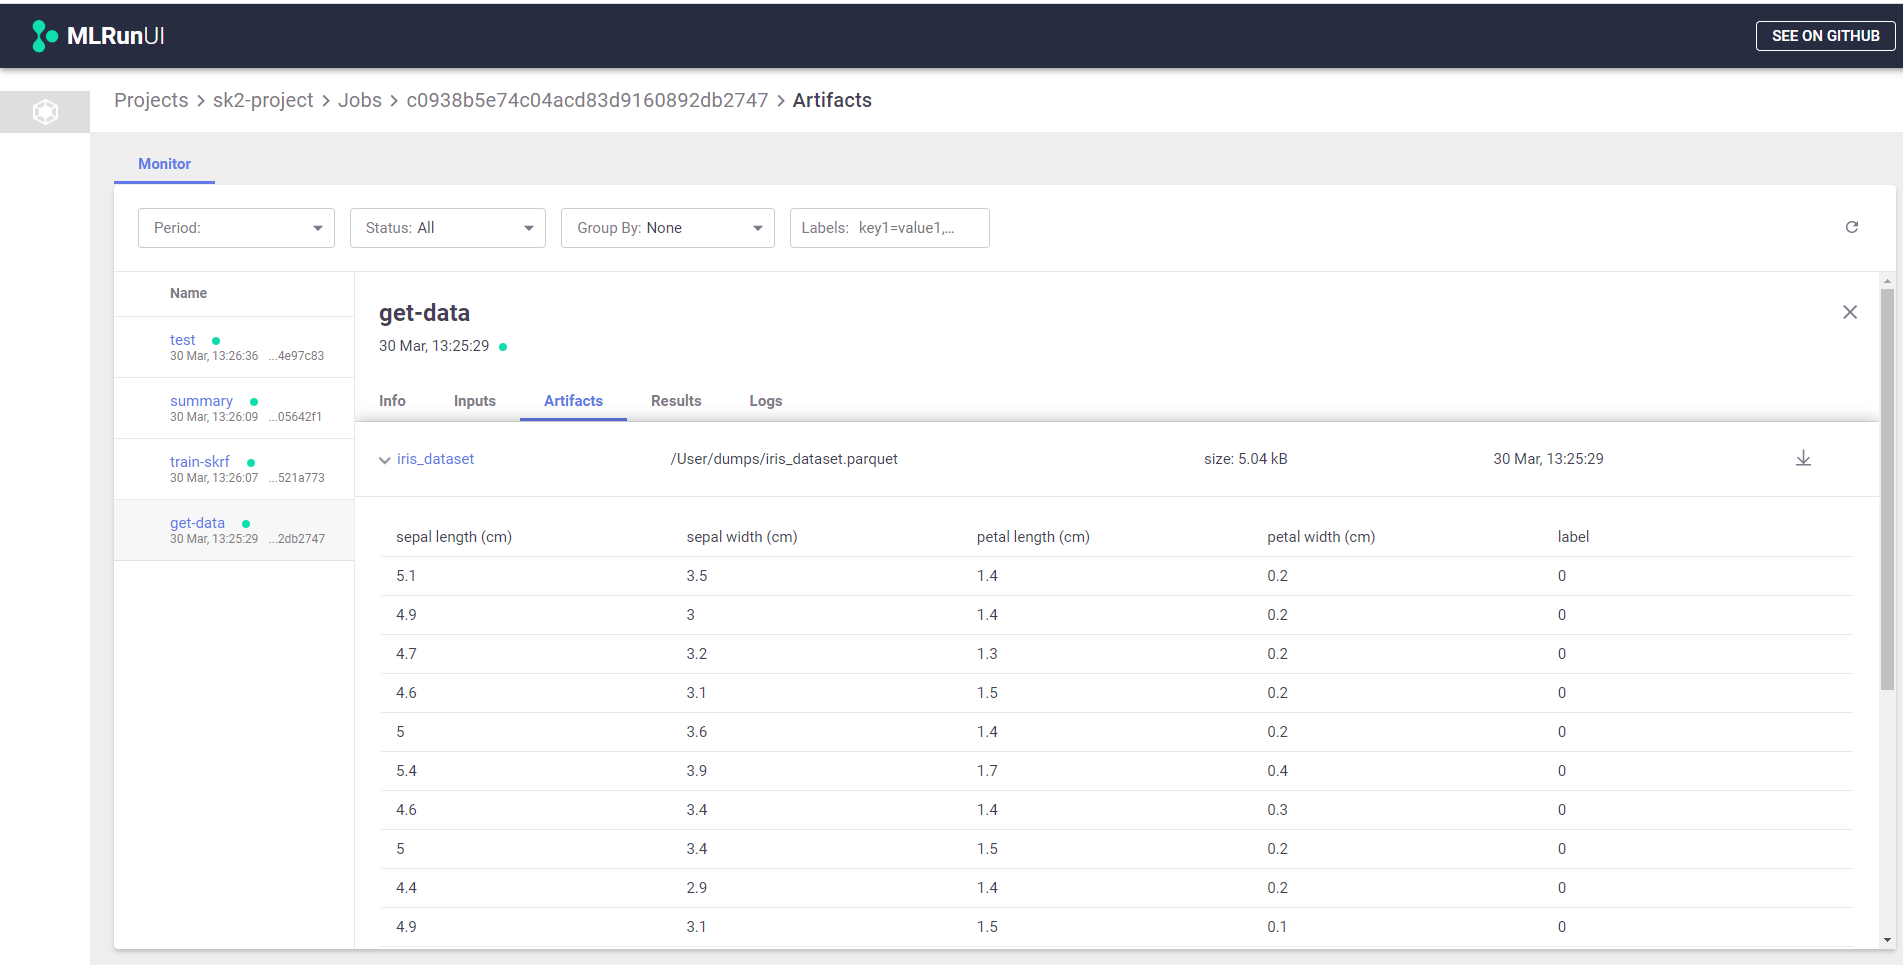
\includegraphics[width=13cm,height=13cm,keepaspectratio]{MLRun Dashbord}
    \end{center}
    \caption{MLRun Dashbord}
    \label{fig:MLRun-dashbord}
\end{figure}

\chapter{Conclusioni}
In questo lavoro di tesi, quindi, ho cercato di capire se fosse possibile l'automazione di pipeline di Machine Learing al fine di trovare uno o più framework che possano essere integrabili con una piattaforma che gestisce risorse/progetti di Machine Learning, come AI4EU.\\
Abbiamo utilizzato un approccio bottom-up, analizzando due casi studio a piacimento. Dopo aver visionato differenti articoli ed estrapolato un workflow per ogni caso, siamo andati ad analizzare le invarianti tra i vari approcci proposti in letteratura.\\
Abbiamo notato come il focus dei diversi approcci trovati può essere differente: alcuni si focalizzano sui dati, ovvero raccolta e pretrattamento, altri invece si focalizzano sulla parte del modello, ovvero costruzione, addestramento e testing.\\
Nel primo caso (AI in radiology) i dati hanno sempre la stessa struttura e c'è anche la possibilità che venga eseguito un aumento del set di dati per la poca disponibilità, ma c'è un grande lavoro di pretrattamento da fare, dato che la qualità delle immagini è fondamentale in questo campo. Il modello è poco versatile: abbiamo sempre trovato una CNN per l'estrazione delle caratteristiche da un'immagine e quasi sempre l'utilizzo di un RNN (preferibilmente una LSTM) per l'estrazione delle parole dalle caratteristiche.\\
Nel secondo caso (Demand forecasting) i dati sono principalmente dati storici e possono avere strutture totalmente differenti, soprattutto in base all'obiettivo della predizione e al tipo di modello utilizzato, con pochissimo pretrattamento dei dati se non riduzione del set di dati. Il modello è molto versatile: come abbiamo già visto, ci sono svariati modelli che possono essere utilizzati e nell'ultimo periodo le reti neurali stanno prendendo sempre più piede.\\
Anche facendo una piccola analisi da un punto di vista cronologico, in generale, il focus si sta spostando sempre di più sull'analisi dei modelli (sul confronto dei modelli) che si utilizzano e sempre meno sul preprocessamento dei dati, ed è proprio per questo che si stanno utilizzando sempre di più le reti neurali, per la loro capacità di integrare informazioni che ho nel data set all'interno del modello.

Sono andato poi alla ricerca di qualche framework per capire se fosse possibile implementare la pipeline e quindi cercare una soluzione che comprenda tutte quante le diverse proprietà e i diversi attributi dei casi specifici.\\
Abbiamo selezionato tre framework molto simili tra loro ma con qualche piccola differenza:
\begin{itemize}
    \item MetaFlow
    \item ZenML
    \item MLRun
\end{itemize}

Sono stati selezionati questi invece che altri soprattutto per la facilità della messa in produzione e perché rispecchiavano di più quelli che erano i punti chiave delle pipeline.\\
In conclusione, tutte le risorse di AI/ML devono essere automatizzate per permetterne l'uso, altrimenti sarebbero inutilizzabili, e grazie a framework come quelli sopra citati è possibile la loro integrazione con una piattaforma già esistente (es: AI4EU).


\chapter*{Appendice} 
\addcontentsline{toc}{chapter}{Appendice}
\section*{Recurrent neural network} 
\label{appendix:RNN}
Una rete neurale ricorrente (recurrent neural network, RNN) è una classe di rete neurale artificiale che include neuroni collegati tra loro in un loop. Tipicamente i valori di uscita di uno strato di un livello superiore sono utilizzati in ingresso di uno strato di livello inferiore. Quest'interconnessione tra strati permette l'utilizzo di uno degli strati come memoria di stato, e consente, fornendo in ingresso una sequenza temporale di valori, di modellarne un comportamento dinamico temporale dipendente dalle informazioni ricevute agli istanti di tempo precedenti. In altri casi lo strato è costituito da un insieme di neuroni dotato di loop di connessioni molto sparse che innesca una dinamica caotica, impiegata per l'addestramento di una parte successiva della rete, come avviene per le echo state network. Ciò le rende applicabili a compiti di analisi predittiva su sequenze di dati, quali possono essere ad esempio il riconoscimento della grafia o il riconoscimento vocale. \cite{itwiki:120617040}

\section*{Convolutional neural network}
\label{appendix:CNN}
Nell'apprendimento automatico, una rete neurale convoluzionale (CNN o ConvNet dall'inglese convolutional neural network) è un tipo di rete neurale artificiale feed-forward in cui il pattern di connettività tra i neuroni è ispirato dall'organizzazione della corteccia visiva animale, i cui neuroni individuali sono disposti in maniera tale da rispondere alle regioni di sovrapposizione che tassellano il campo visivo. Le reti convoluzionali sono ispirate da processi biologici e sono variazioni di percettroni multistrato progettate per usare al minimo la preelaborazione. Hanno diverse applicazioni nel riconoscimento di immagini e video, nei sistemi di raccomandazione, nell'elaborazione del linguaggio naturale e, recentemente, in bioinformatica. \cite{itwiki:122354896}
    
\section*{Long-Short Term Memory}
\label{appendix:LSTM}
La memoria a lungo termine (LSTM) è un'architettura di rete neurale ricorrente artificiale (RNN) utilizzata nel campo dell'apprendimento profondo. A differenza delle reti neurali feedforward standard, LSTM ha connessioni di feedback. Può elaborare non solo singoli punti dati (come immagini), ma anche intere sequenze di dati (come voce o video). Ad esempio, LSTM è applicabile ad attività come il riconoscimento della scrittura non segmentato e connesso, il riconoscimento vocale e il rilevamento di anomalie nel traffico di rete o IDS (sistemi di rilevamento delle intrusioni). \cite{enwiki:1046770680}

\begin{figure}[h!]
    \begin{center}
        \includegraphics[width=7cm,height=7cm,keepaspectratio]{diagram_LSTM}
    \end{center}
    \caption{Schema di una cella LSTM}
    \label{fig:LSTM-schema}
\end{figure}

\section*{Gated Recurrent Units (GRU)}
\label{appendix:GRU}
Le Gated Recurrent Units (GRU) sono un meccanismo di gating nelle reti neurali ricorrenti, introdotto nel 2014 da Kyunghyun Cho et al. Il GRU è come una memoria a lungo termine (LSTM) con un cancello di dimenticanza, ma ha meno parametri di LSTM, poiché manca un cancello di uscita. Le prestazioni del GRU su alcuni compiti di modellazione della musica polifonica, della modellazione del segnale vocale e dell'elaborazione del linguaggio naturale sono risultate simili a quelle di LSTM.

\section*{Natural language processing (NLP)}
\label{appendix:NLP}
L'elaborazione del linguaggio naturale (in inglese: natural language processing, in acronimo: NLP) è il processo di trattamento automatico mediante un calcolatore elettronico delle informazioni scritte o parlate in una lingua.

\section*{Neuro-linguistic programming (PNL)}
\label{appendix:PNL}
La programmazione neurolinguistica (PNL; in inglese neuro-linguistic programming, NLP) è un metodo di comunicazione e un sistema di "life coaching", "self-help" e "counseling", definito da alcuni suoi promotori come «un approccio alla comunicazione, allo sviluppo personale e alla psicoterapia.

\section*{Power Trasformation (Box-Cox)}
\label{appendix:Box-Cox}
In statistica, una trasformazione di potenza è una famiglia di funzioni applicate per creare una trasformazione monotona di dati utilizzando le funzioni di potenza. È una tecnica di trasformazione dei dati utilizzata per stabilizzare la varianza, rendere i dati più normali come una distribuzione, migliorare la validità delle misure di associazione (come la correlazione di Pearson tra le variabili) e per altre procedure di stabilizzazione dei dati.\\
Le trasformazioni di potenza sono utilizzate in più campi, tra cui analisi multi-risoluzione e wavelet, analisi dei dati statistici, ricerca medica, modellazione di processi fisici, analisi dei dati geochimici, epidemiologia e molti altri clinici, aree di ricerca ambientale e sociale.

\section*{Distribuzione di probabilità a priori}
\label{appendix:prior}
Nell'ambito dell'inferenza statistica bayesiana, una distribuzione di probabilità a priori, detta spesso anche distribuzione a priori, di una quantità incognita p è la distribuzione di probabilità che esprimerebbe l'incertezza di p prima che i "dati" siano presi in considerazione. Il proposito è di attribuire incertezza piuttosto che casualità a una quantità incerta.

\section*{Docker}
\label{appendix:Docker}
Docker è un progetto open-source che automatizza il processo di deployment di applicazioni all'interno di contenitori software, fornendo un'astrazione aggiuntiva grazie alla virtualizzazione a livello di sistema operativo di Linux.\cite{itwiki:123095653}

\section*{Kubernetes}
\label{appendix:Kubernetes}
Kubernetes (abbreviato K8s) è un sistema open-source di orchestrazione e gestione di container. Inizialmente sviluppato da Google, adesso è mantenuto da Cloud Native Computing Foundation. Funziona con molti sistemi di containerizzazione, compreso Docker.\cite{itwiki:119581182}

\section*{Exponential Smoothing di Holt Winter}
\label{appendix:ETS}
L'Exponential Smoothing di Holt Winter. Holt (1957) e Winters (1960) ha esteso il metodo di Holt per catturare la stagionalità. Il metodo stagionale di Holt- Winters comprende l'equazione di previsione e tre equazioni di livellamento: una per il livello \textit{ltlt}, una per l'andamento bt e una per la componente stagionale st, con i corrispondenti parametri di livellamento $\alpha\alpha$ , $\beta*\beta*$ e $\gamma\gamma$. Usiamo $mm$ per indicare la frequenza della stagionalità, cioè il numero di stagioni in un anno. Ad esempio, per i dati trimestrali $m=4m=4$ e i dati mensili $m=12m=12$.
Esistono due varianti di questo metodo che differiscono come la componente stagionale. Il metodo additivo è preferito quando le variazioni stagionali sono grosso modo costanti lungo la serie, mentre il metodo moltiplicativo è preferito quando le variazioni stagionali cambiano proporzionalmente al livello della serie. Con il metodo additivo la componente stagionale è espressa in termini assoluti nella scala della serie osservata e nell'equazione di livello la serie è destagionalizzata sottraendo la componente stagionale. All'interno di ogni anno, la componente stagionale raggiungerà approssimativamente lo zero. Con il metodo moltiplicativo la componente stagionale è espressa in termini relativi (percentuali) e la serie è destagionalizzata dividendo per la componente stagionale. All'interno di ogni anno, la componente stagionale si sommerà a circa mm.

\section*{ARIMA/SARIMA}
\label{appendix:ARIMA}
ARIMA, abbreviazione di "Auto-Regressive Integrated Moving Average" (Media mobile integrata auto-regressiva), è in realtà una classe di modelli che "spiega" una determinata serie temporale in base ai propri valori passati, ovvero i propri ritardi e gli errori di previsione ritardati, in modo che l'equazione possa essere utilizzato per prevedere i valori futuri. Qualsiasi "serie temporale non stagionale che mostra modelli e non è un rumore bianco casuale" può essere modellata con i modelli ARIMA. Le serie temporali sono una sequenza di punti dati presi in punti temporali successivi equidistanti. Le principali componenti da analizzare sono: trend, stagionalità, irregolarità, ciclicità.
I modelli ARIMA mirano, quindi, a descrivere le autocorrelazioni nei dati delle serie temporali. Quando si pianificano previsioni a breve termine, ARIMA può fare previsioni accurate. Fornendo valori previsti per periodi specificati dall'utente, mostra chiaramente i risultati per domanda, vendite, pianificazione e produzione.

Un modello ARIMA è caratterizzato da 3 termini: p, d, q dove,
\begin{itemize}
    \item p è l'ordine del termine AR
    \item q è l'ordine del termine MA
    \item d è il numero di differenze necessarie per rendere stazionaria la serie storica
\end{itemize}

Se una serie temporale ha modelli stagionali, è necessario aggiungere termini stagionali e diventa SARIMA, abbreviazione di "Seasonal ARIMA". 

\section*{Root-mean-square deviation (RMSD)}
\label{appendix:RMSD}
La deviazione quadratica media (RMSD) o errore quadratico medio (RMSE) è una misura utilizzata di frequente delle differenze tra i valori (campioni o valori della popolazione) previsti da un modello o da uno stimatore e i valori osservati. L'RMSD rappresenta la radice quadrata del secondo momento campionario delle differenze tra valori previsti e valori osservati o la media quadratica di queste differenze. Queste deviazioni sono chiamate residui quando i calcoli vengono eseguiti sul campione di dati utilizzato per la stima e sono chiamate errori (o errori di previsione) quando vengono calcolati fuori campione. L'RMSD serve ad aggregare le grandezze degli errori nelle previsioni per vari punti dati in un'unica misura del potere predittivo. RMSD è una misura di accuratezza, per confrontare gli errori di previsione di diversi modelli per un particolare set di dati e non tra set di dati, poiché dipende dalla scala.

\section*{Mean absolute percentage error (MAPE)}
\label{appendix:MAPE}
L'errore percentuale medio assoluto (MAPE), noto anche come deviazione percentuale media assoluta (MAPD), è una misura dell'accuratezza della previsione di un metodo di previsione nelle statistiche. Di solito esprime l'accuratezza come un rapporto definito dalla formula:
\begin{equation}
    {\displaystyle MAPE = \frac{100}{n} \sum\limits_{t=1}^{n} \vert \frac{A_t - F_t}{A_t} \vert}
\end{equation}

dove $A_t$ è il valore effettivo e $F_t$ è il valore previsto. La loro differenza viene divisa per il valore effettivo $A_t$. Il valore assoluto in questo rapporto viene sommato per ogni momento previsto e diviso per il numero di punti montati $n$.

\section*{DICOM}
\label{appendix:DICOM}
DICOM (Digital Imaging and COmmunications in Medicine, immagini e comunicazione digitali in medicina) è uno standard che definisce i criteri per la comunicazione, la visualizzazione, l'archiviazione e la stampa di informazioni di tipo biomedico quali ad esempio immagini radiologiche.

\section*{PACS}
\label{appendix:PACS}
PACS è l'acronimo anglosassone di Picture archiving and communication system (sistema di archiviazione e trasmissione di immagini) e consiste in un sistema hardware e software dedicato all'archiviazione, trasmissione, visualizzazione e stampa delle immagini diagnostiche digitali.


\nocite{*}
\bibliographystyle{plain}
\bibliography{Bibliography}

\chapter*{Ringraziamenti}
Questo spazio lo dedico alle persone che, con il loro supporto, mi hanno aiutato in questi tre anni.\\
Vorrei innanzitutto ringraziare il mio relatore prof. Maurizio Gabbrielli, che mi ha immesso nel mondo dell'AI e mi ha seguito in questo percorso.\\
Grazie anche ai miei correlatori Stefano Pio Zingaro e Saverio Giallorenzo, per avermi guidato, per i loro preziosi consigli e per l'infinta pazienza.\\
Ringrazio infinitamente mia madre: senza il suo supporto, i suoi insegnamenti e sopratutto senza tutti i suoi sacrifici, questo lavoro di tesi non esisterebbe nemmeno.\\
Ringrazio mia sorella, per avermi supportato e sopportato durante questo periodo e nei momenti bui. Senza di lei non sarei quello che sono.\\
Ringrazio Marco e Simone che oltre ad essere miei compagni di corso sono stati anche la mia salvezza nella stesura di questa tesi. Abbiamo iniziato e finito insieme questo viaggio e spero che il prossimo sarà altrettanto bello.\\
Ringrazio anche gli altri miei colleghi, Enea, Riccardo, Matteo, Gabriele, Paolo, Mirko e Damiano: senza il loro aiuto, senza i momenti insieme non sarebbe stato facile affrontare questi tre anni.\\
Ringrazio di cuore tutti i miei amici per tutto il loro supporto in questo viaggio un po' stressante, ci siete sempre stati.\\
Infine, vorrei dedicare questo elaborato, questo mio percorso al mio angelo custode: papà. Anche se non sei più qui, ti sento più vicino che mai e spero di averti reso orgoglioso di me.\\

\end{document}